\chapter{Analisi dei requisiti}
\label{chap:analisi-requisiti}

\section{Panoramica e Attori}
\noindent Come illustrato nel capitolo introduttivo, il progetto di stage mira a estendere l'ecosistema \gls{ergteam} con una nuova funzionalità dedicata alla gestione delle note spesa. Poiché l'applicativo base risulta già consolidato e provvisto di funzionalità cardine come il processo di autenticazione e la navigazione principale, la presente analisi dei requisiti si focalizzerà esclusivamente sul nuovo dominio applicativo. Di conseguenza, i flussi preesitenti verranno considerati come parte integrante del sistema, e non saranno oggetto di analisi dettagliata in questa fase. 

\subsection{Attori del sistema}
\noindent Gli attori rappresentano le entità (utenti fisici o sistemi esterni) che interagiscono con l'applicazione. Per il progetto sviluppato, sono stati individuati i seguenti attori principali:
\begin{itemize}
    \item \textbf{Dipendente (Utente):} rappresenta un dipendente dell'azienda che ha già effettuato l'accesso all'applicazione \gls{ergteam} tramite le proprie credenziali. Esso interagisce con la nuova sezione per consultare lo storico delle proprie spese inserite e per inserire nuove note spesa da inoltrare al sistema.
    
    \item \textbf{Azure Content Understanding (Sistema di IA):} sistema esterno basato su intelligenza artificiale, interrogato dall'applicazione per l'estrazione automatica dei dati dalle fotografie degli scontrini, al fine di semplificare e velocizzare la compliazione della nota spesa da parte del dipendente.
\end{itemize}




\section{Casi d'uso}
\noindent I diagrammi dei casi d'uso (Use Case Diagram) sono diagrammi di tipo \gls{uml} dedicati alla descrizione delle funzioni offerte da un sistema, così come sono percepite e utilizzate dagli attori che interagiscono con il sistema stesso. Di seguito verranno descritti nel dettaglio i casi d'uso relativi all'integrazione del modulo "Note spesa" all'interno dell'applicazione mobile aziendale. \newline
Ognuno dei casi d'uso seguirà la seguente struttura:
\begin{itemize}
          \item \textbf{Caso d'uso}: codice e nome del caso d'uso;
          \item \textbf{Attori}: attori dello scenario;
          \item \textbf{Descrizione}: descrizione dettagliata del caso d'uso, con i passaggi che lo caratterizzano;
          \item \textbf{Precondizioni}: condizioni che devono essere soddisfatte affinché l'attore possa accedere al caso d'uso;
          \item \textbf{Postcondizioni}: stato del sistema dopo che il caso d'uso si è verificato;
          \item \textbf{Scenario principale}: sequenza di passi che descrivono il flusso principale del caso d'uso, ovvero la sequenza di azioni che si verificano quando tutto va come previsto;
          \item \textbf{Scenario alternativo}: eventuali scenari alternativi che possono verificarsi durante l'esecuzione del caso d'uso, con le relative condizioni e conseguenze.
      \end{itemize} 

\begin{figure}[H]
    \vspace{2em}
    \centering
    \includegraphics[alt={Note spesa: schermata principale}, width=0.95\columnwidth]{img/usecase/Ucprinc.jpg}
    \caption{Note spesa: Schermata principale}
    \label{fig:schermata_principale}
\end{figure}

\begin{usecase}{1}{Visualizzazione lista resoconti mensili}
    \begin{figure}[H]
        \vspace{2em}
        \centering
        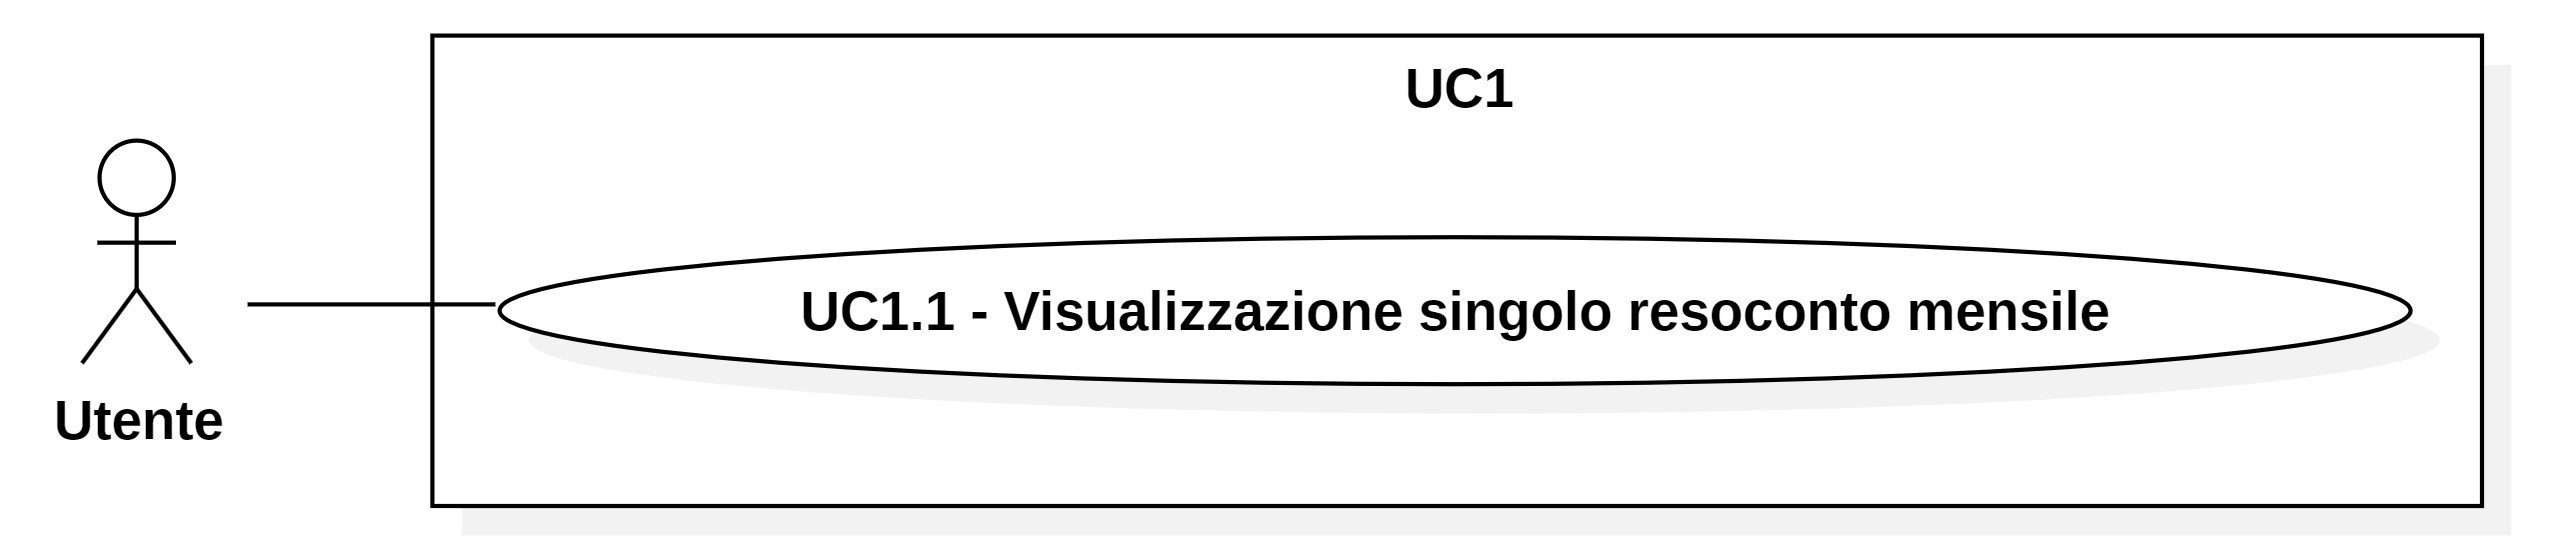
\includegraphics[alt={Use Case 1: Visualizzazione lista resoconti mensili}, width=0.90\columnwidth]{img/usecase/UC1.jpg}
        \caption{UC1: Visualizzazione lista resoconti mensili}
        \label{fig:UC1}
    \end{figure}
    \usecaseactors{Utente.}
    \usecasedesc{L'utente visualizza la lista dei resoconti mensili relativi alle note spesa presenti nel sistema.}
    \usecasepre{L'utente ha effettuato l'accesso all'applicazione e ha navigato nella sezione dedicata alle note spesa.}
    \usecasepost{La schermata iniziale con la lista dei resoconti mensili viene mostrata correttamente.}
    \usecaseprin{
        \begin{itemize}
            \item L'utente accede alla schermata principale del modulo.
            \item Il sistema recupera i resoconti mensili disponibili.
            \item L'utente visualizza la lista dei resoconti mensili delle proprie note spesa, con le informazioni di riepilogo.
        \end{itemize}
    }
    \usecasealt{
        \begin{itemize}
            \item Se non sono presenti note spesa, il sistema mostra un messaggio informativo.
        \end{itemize}   
    }
    \label{uc:uc_visualizzazione_lista_resoconti_mensili}
\end{usecase}

\begin{usecase}{1.1}{Visualizzazione singolo resoconto mensile}
    \usecaseactors{Utente.}
    \usecasedesc{Il sistema mostra un singolo resoconto mensile nella lista dei resoconti mensili disponibili.}
    \usecasepost{Il sistema mostra il singolo resoconto mensile con le informazioni di riepilogo.}
    \usecaseprin{
        \begin{itemize}
            \item Viene visualizzato il singolo resoconto mensile: sono mostrati il mese, l'anno, l'importo totale, il numero di note spesa del resoconto e l'eventuale indicatore di note spesa non sincronizzate.
        \end{itemize}
    }
    \label{uc:uc_visualizzazione_singolo_resoconto}
\end{usecase}

\begin{usecase}{2}{Filtro resoconti per anno}
    \usecaseactors{Utente.}
    \usecasedesc{L'utente filtra la lista dei resoconti mensili visualizzando solo quelli appartenenti a un determinato anno selezionato.}
    \usecasepre{L'utente visualizza la schermata iniziale.}
    \usecasepost{Il sistema mostra all'utente la lista aggiornata contenente esclusivamente i resoconti mensili relativi all'anno scelto.}
    \usecaseprin{
        \begin{itemize}
            \item L'utente preme l'apposito tasto per selezionare l'anno per cui filtrare i resoconti.
            \item Il sistema mostra la lista degli anni selezionabili e la voce "Tutti".
            \item L'utente seleziona un elemento dalla lista.
            \item Il sistema aggiorna la lista mostrando solo i resoconti corrispondenti alla selezione effettuata.
        \end{itemize}
    }
    \label{uc:uc_filtro_resoconti_anno}
\end{usecase}

\begin{usecase}{3}{Sincronizzazione note spesa locali}
    \begin{figure}[H]
        \vspace{2em}
        \centering
        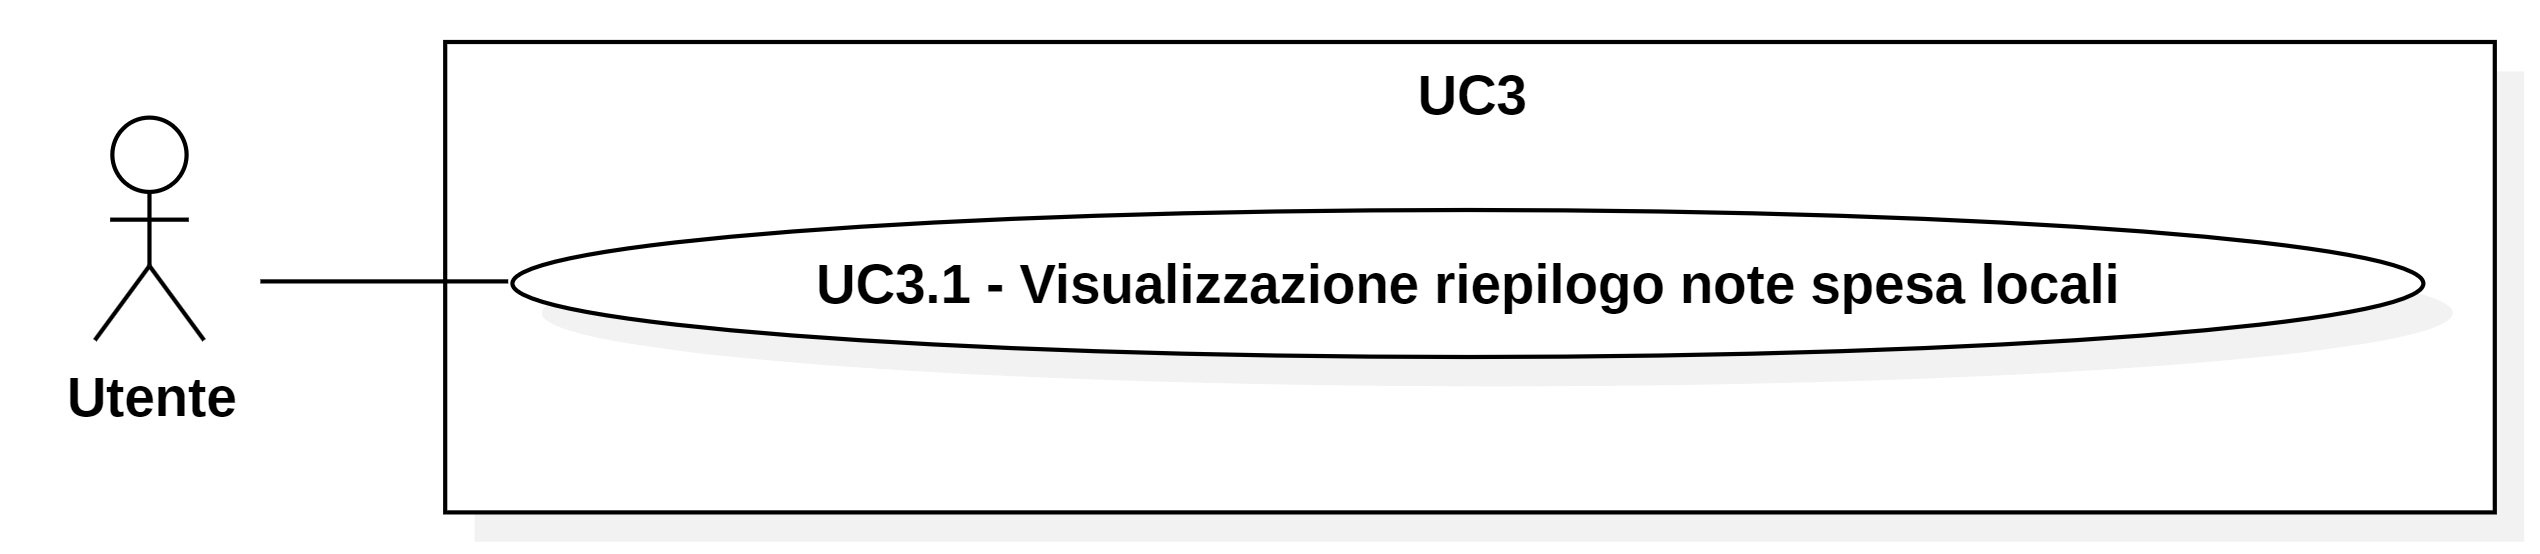
\includegraphics[alt={Use Case 3: Sincronizzazione note spesa locali}, width=0.95\columnwidth]{img/usecase/UC3.jpg}
        \caption{UC3: Sincronizzazione note spesa locali}
        \label{fig:UC3}
    \end{figure}
    \usecaseactors{Utente.}
    \usecasedesc{L'utente vuole inviare al server tutte le note spesa contrassegnate come locali presenti nel sistema.}
    \usecasepre{L'utente visualizza la schermata iniziale ed è presente almeno una nota spesa non sincronizzata nel sistema.}
    \usecasepost{Le note spesa vengono inviate al server, l'interfaccia si aggiorna e vengono rimosse le icone di avviso dai resoconti.}
    \usecaseprin{
        \begin{itemize}
            \item L'utente preme il bottone per effettuare la sincronizzazione.
            \item Il sistema mostra il riepilogo delle note spesa che si apprestano a essere sincronizzate (\ref{uc:uc_visualizzazione_riepilogo_note_sincronizzazione}).
            \item L'utente preme il bottone per confermare l'operazione.
            \item Il sistema aggiorna le note spesa e la lista dei resoconti.
        \end{itemize}
    }
    \usecasealt{
        \begin{itemize}
            \item L'utente preme il bottone per annullare l'operazione.
            \item Il pop-up si chiude e l'utente torna alla schermata principale (\ref{uc:uc_visualizzazione_lista_resoconti_mensili}).
        \end{itemize}
    }
    \label{uc:uc_sincronizzazione_note}
\end{usecase}

\begin{usecase}{3.1}{Visualizzazione riepilogo note spesa locali}
    \usecaseactors{Utente.}
    \usecasedesc{Il sistema mostra, all'interno di un pop-up, un riepilogo dettagliato delle note spesa locali che si apprestano a essere sincronizzate.}
    \usecasepre{L'utente preme il bottone per effettuare la sincronizzazione di tutte le note spesa locali o visualizza il promemoria di note spesa non sincronizzate.}
    \usecasepost{Il sistema rimane in attesa della risposta dell'utente.}
    \usecaseprin{
        \begin{itemize}
            \item Il sistema mostra la finestra modale in sovraimpressione.
            \item Vengono visualizzati i dettagli delle note da sincronizzare, come tipologia, data e importo.
            \item Vengono visualizzati i pulsanti per annullare o confermare l'operazione.
        \end{itemize}
    }
    \label{uc:uc_visualizzazione_riepilogo_note_sincronizzazione}
\end{usecase}

\newpage
\begin{usecase}{4}{Accesso schermata inserimento}
    \begin{figure}[H]
        \vspace{2em}
        \centering
        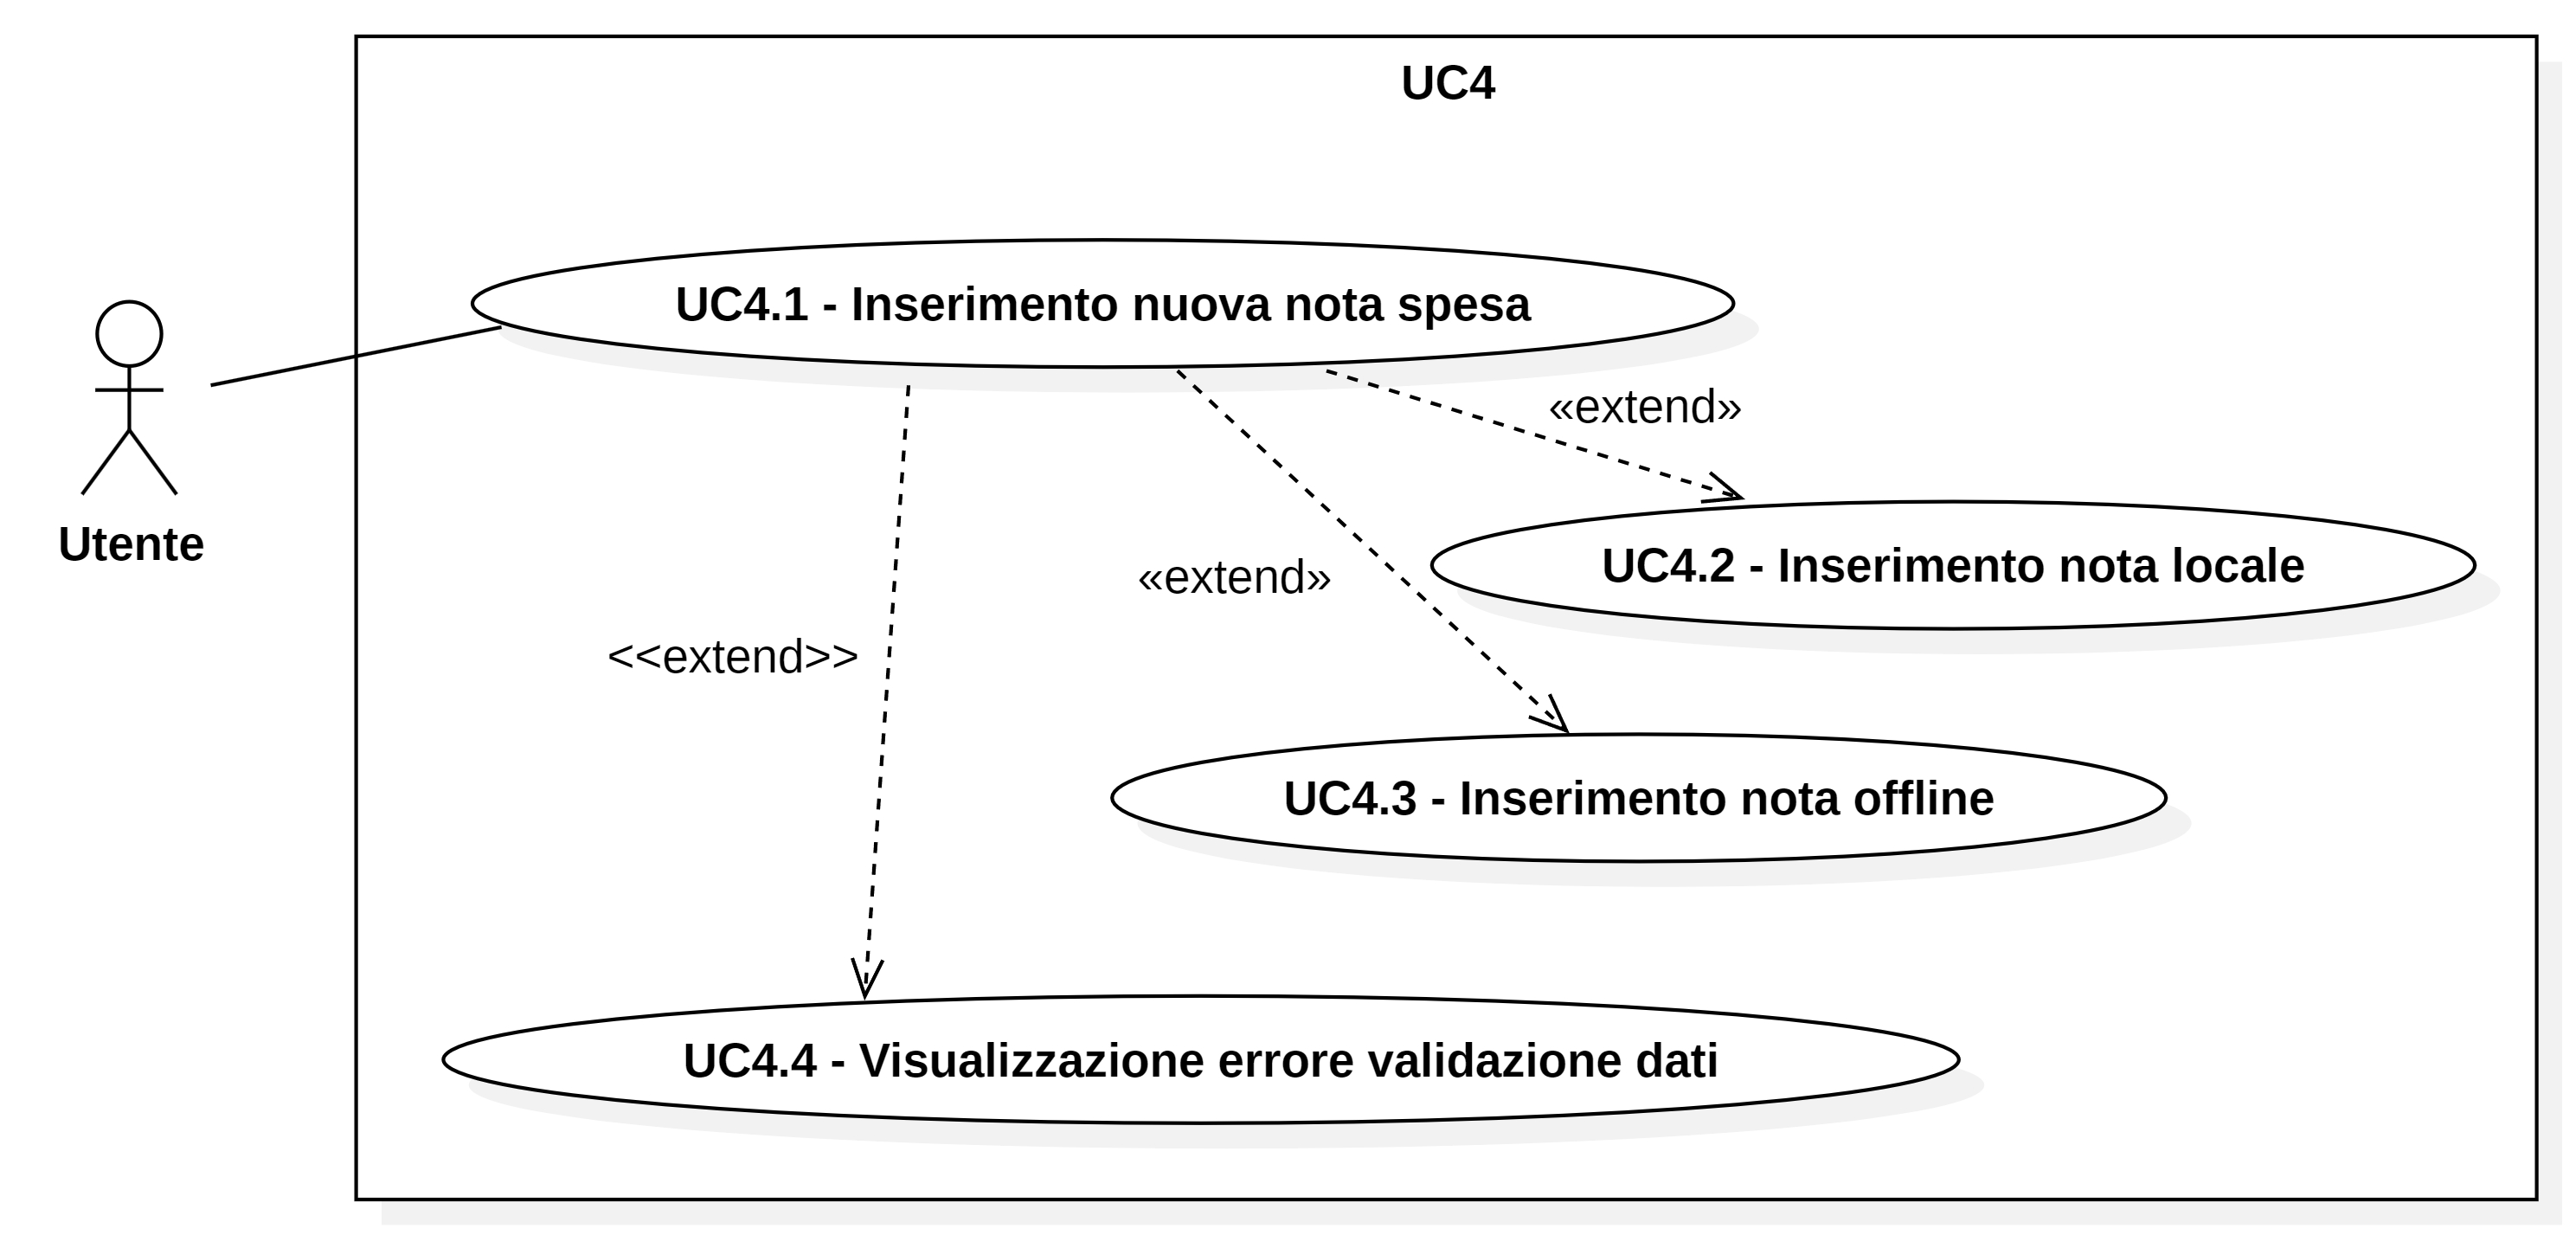
\includegraphics[alt={Use Case 4: Accesso schermata inserimento}, width=1\columnwidth]{img/usecase/UC4.jpg}
        \caption{UC4: Accesso schermata inserimento}
        \label{fig:UC4}
    \end{figure}
    \usecaseactors{Utente.}
    \usecasedesc{L'utente accede alla schermata di inserimento di una nuova nota spesa.}
    \usecasepre{L'utente si trova nella schermata principale o nella schermata di visualizzazione della lista note.}
    \usecasepost{L'utente visualizza la schermata di inserimento di una nuova nota spesa.}
    \usecaseprin{
        \begin{itemize}
            \item L'utente preme il bottone "+" per accedere alla schermata di inserimento.
        \end{itemize}
    }
    \label{uc:uc_accesso_schermata_inserimento}
\end{usecase}

\begin{usecase}{4.1}{Inserimento nuova nota spesa}
    \usecaseactors{Utente, Sistema \gls{ia}.}
    \usecasedesc{L'utente vuole inserire una nuova nota spesa nel sistema.}
    \usecasepre{L'utente ha effettuato l'accesso alla schermata di inserimento di una nuova nota spesa.}
    \usecasepost{La nuova nota spesa viene salvata nel sistema.}
    \usecaseprin{
        \begin{itemize}
            \item L'utente seleziona il cliente associato alla spesa (\ref{uc:uc_selezione_cliente_spesa}).
            \item L'utente inserisce o acquisisce i dati della spesa (\ref{uc:uc_compilazione_dati_generali_spesa}).
            \item Il sistema valida i dati inseriti.
            \item L'utente conferma il salvataggio della nota.
            \item Il sistema salva la nota.
        \end{itemize}
    }
    \usecasealt{
        \begin{itemize}
            \item \textbf{Validazione dati:} il sistema segnala errori nei dati inseriti e interrompe il salvataggio (\ref{uc:uc_errore_validazione_nota}).
            \item \textbf{Assenza connessione:} se il dispositivo è offline, la nota viene salvata localmente con stato "locale" (\ref{uc:uc_inserimento_nota_locale}).
        \end{itemize}
    }
    \label{uc:uc_inserimento_nuova_nota_spesa}
\end{usecase}

\begin{usecase}{4.2}{Inserimento nota locale}
    \usecaseactors{Utente.}
    \usecasedesc{L'utente vuole inserire una nuova nota spesa locale nel sistema.}
    \usecasepre{L'utente ha effettuato l'accesso alla schermata di inserimento di una nuova nota spesa.}
    \usecasepost{La nuova nota spesa locale viene salvata nel sistema.}
    \usecaseprin{
        \begin{itemize}
            \item L'utente inserisce tutti i campi obbligatori per la creazione di una nuova nota spesa.
            \item L'utente seleziona l'opzione "Posticipa caricamento".
            \item L'utente preme il pulsante "SALVA NOTA" per confermare l'inserimento.
        \end{itemize}
    }
    \label{uc:uc_inserimento_nota_locale}
\end{usecase}

\begin{usecase}{4.3}{Inserimento nota offline}
    \usecaseactors{Utente.}
    \usecasedesc{L'utente vuole inserire una nuova nota spesa nel sistema.}
    \usecasepre{L'utente ha inserito tutti i campi obbligatori e non ha selezionato l'opzione "Posticipa caricamento", ma il dispositivo è offline.}
    \usecasepost{La nuova nota spesa viene salvata nel sistema come nota locale.}
    \usecaseprin{
        \begin{itemize}
            \item L'utente preme il pulsante "SALVA NOTA" per confermare l'inserimento.
        \end{itemize}
    }
    \label{uc:uc_inserimento_nota_offline}
\end{usecase}

\begin{usecase}{4.4}{Visualizzazione errore validazione dati}
    \usecaseactors{Utente.}
    \usecasedesc{L'utente tenda di salvare una nota spesa con campi non compilati correttamente.}
    \usecasepre{L'utente ha premuto "SALVA NOTA" avendo omesso dati obbligatori o avendo inserito dati in formati non validi.}
    \usecasepost{Il salvataggio è interrotto e l'utente rimane sulla schermata di inserimento.}
    \usecaseprin{
        \begin{itemize}
            \item La logica di validazione individua l'assenza di uno o più campi obbligatori.
            \item Il sistema interrompe l'operazione di salvataggio.
            \item Il sistema mostra a schermo uno o più alert specifici indicanti l'errore.
        \end{itemize}
    }
    \label{uc:uc_errore_validazione_nota}
\end{usecase}

\begin{figure}[H]
    \vspace{2em}
    \centering
    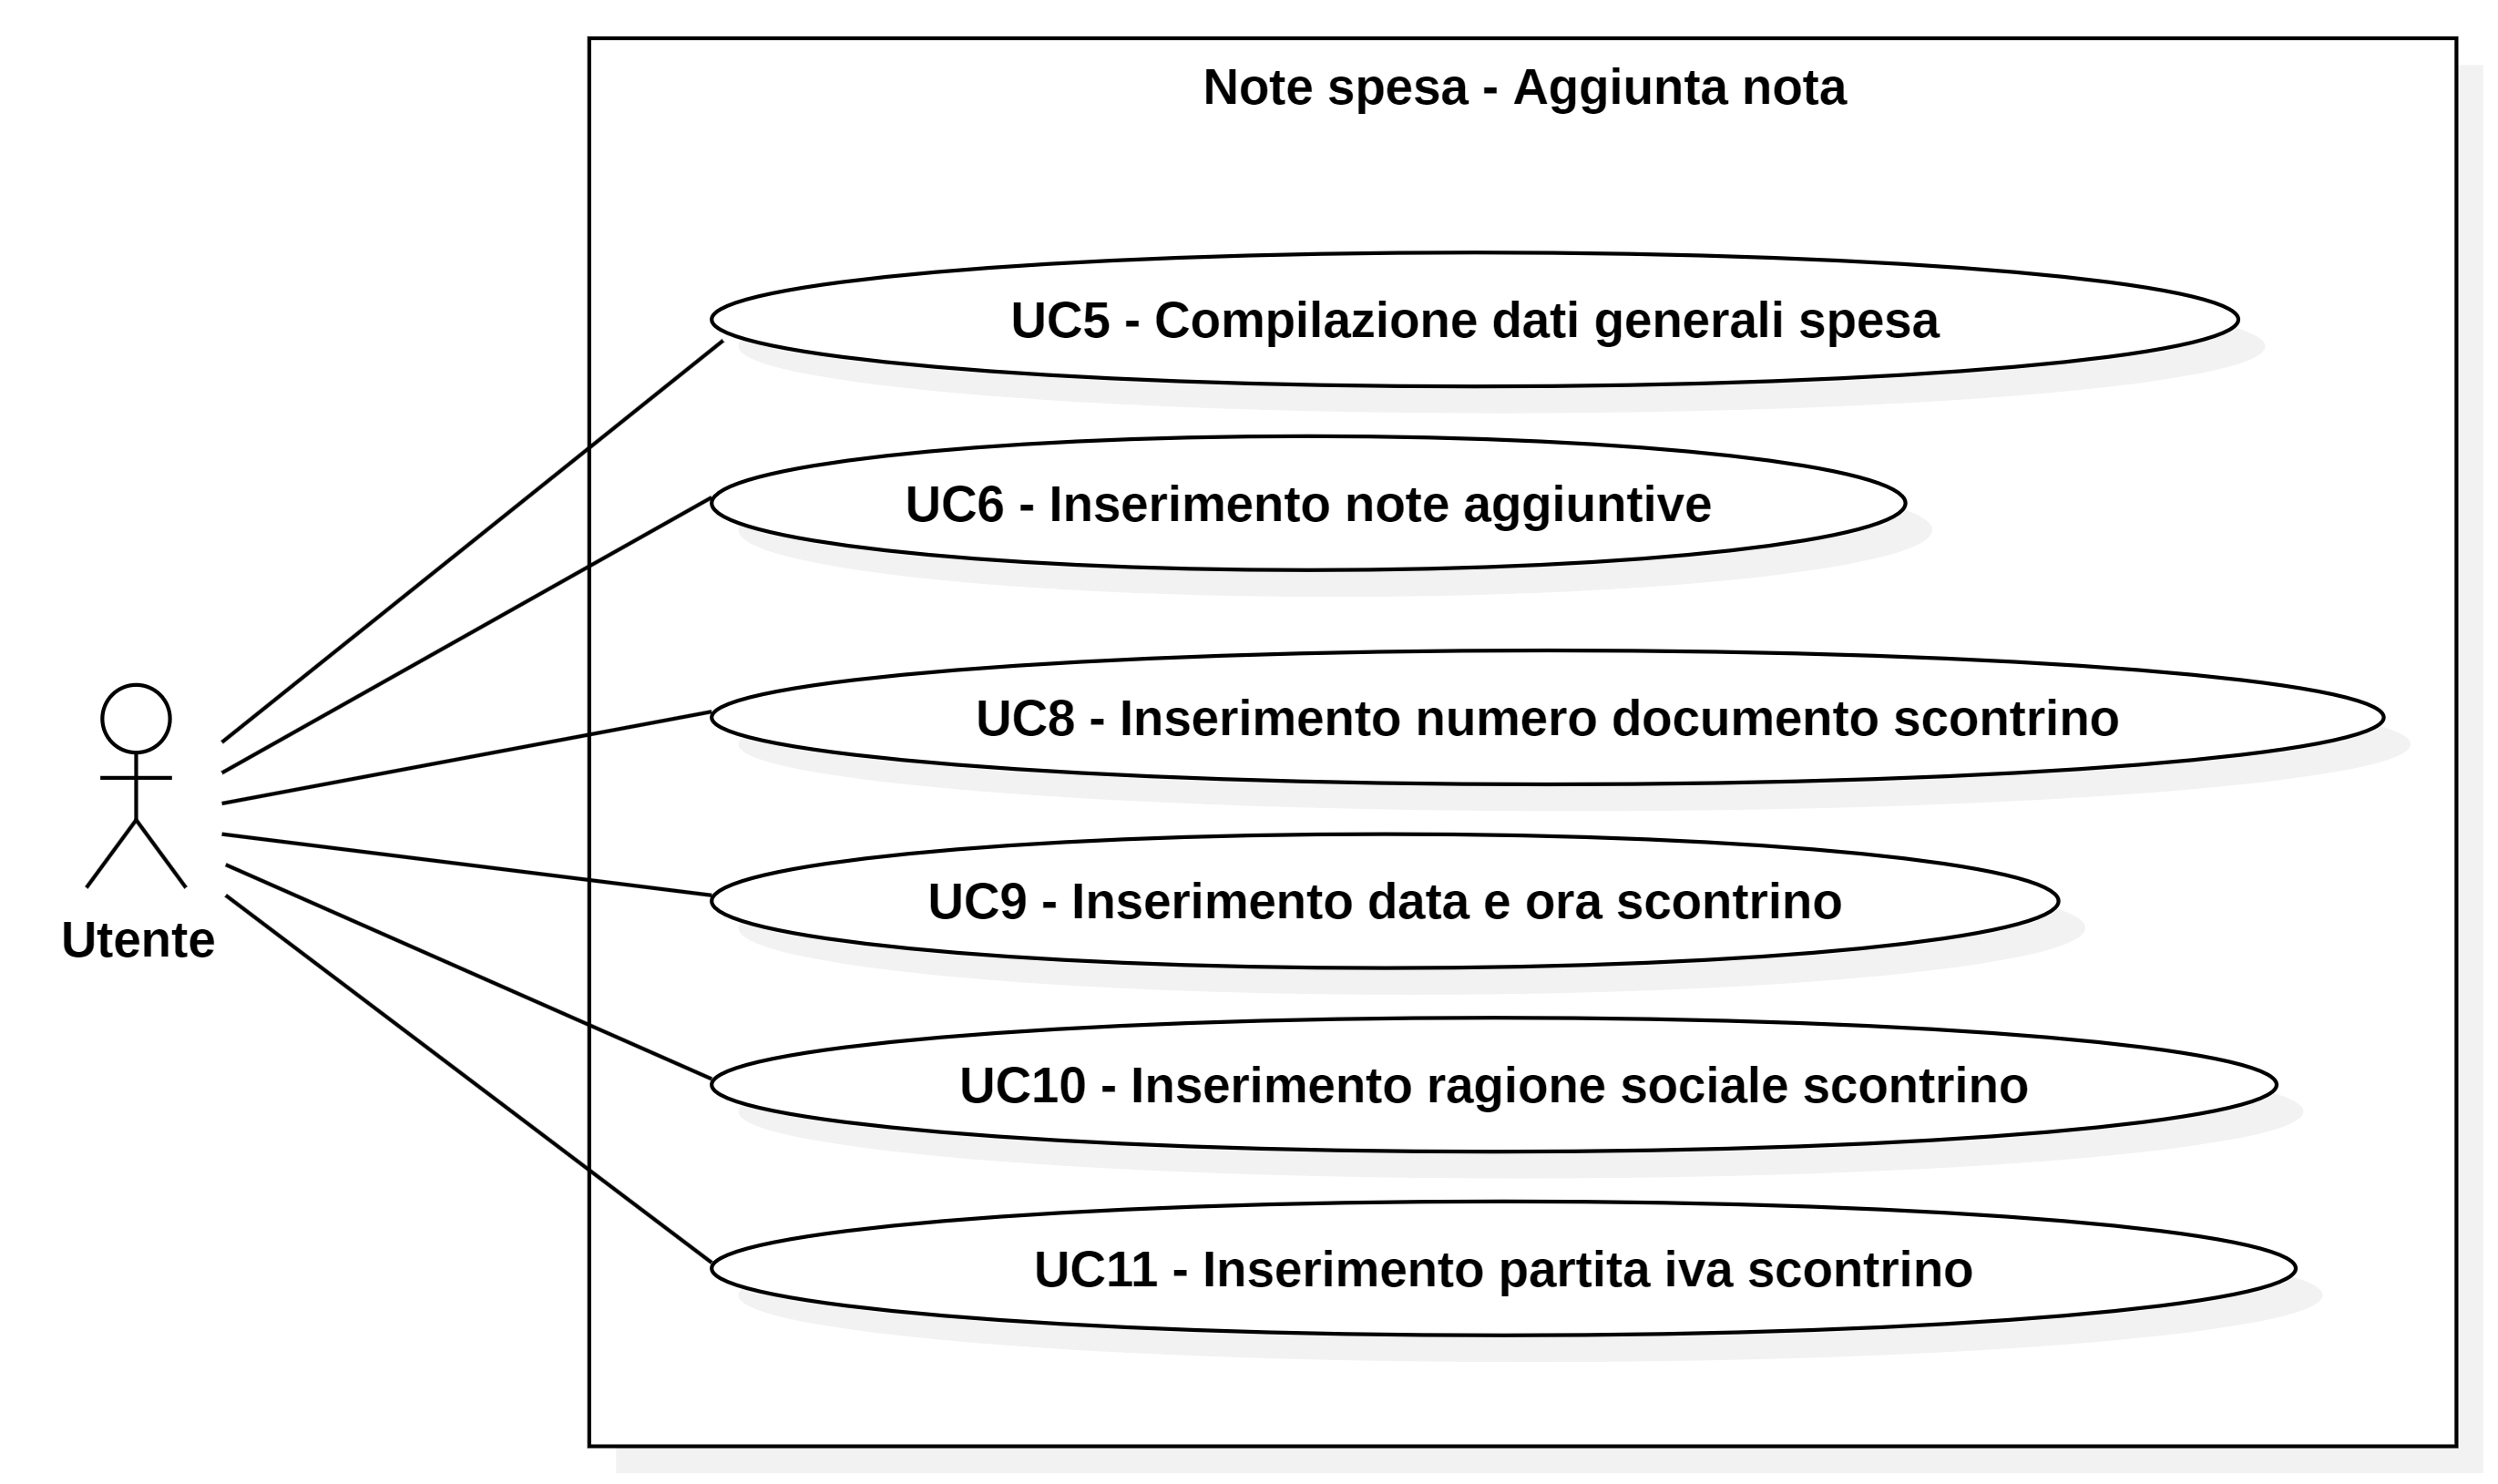
\includegraphics[alt={Scenario di aggiunta di una nota spesa}, width=0.95\columnwidth]{img/usecase/UCAggiunta.jpg}
    \caption{Nota spesa: Aggiunta nota}
    \label{fig:UCAggiunta}
\end{figure}

\begin{usecase}{5}{Compilazione dati generali spesa}
    \begin{figure}[H]
        \vspace{2em}
        \centering
        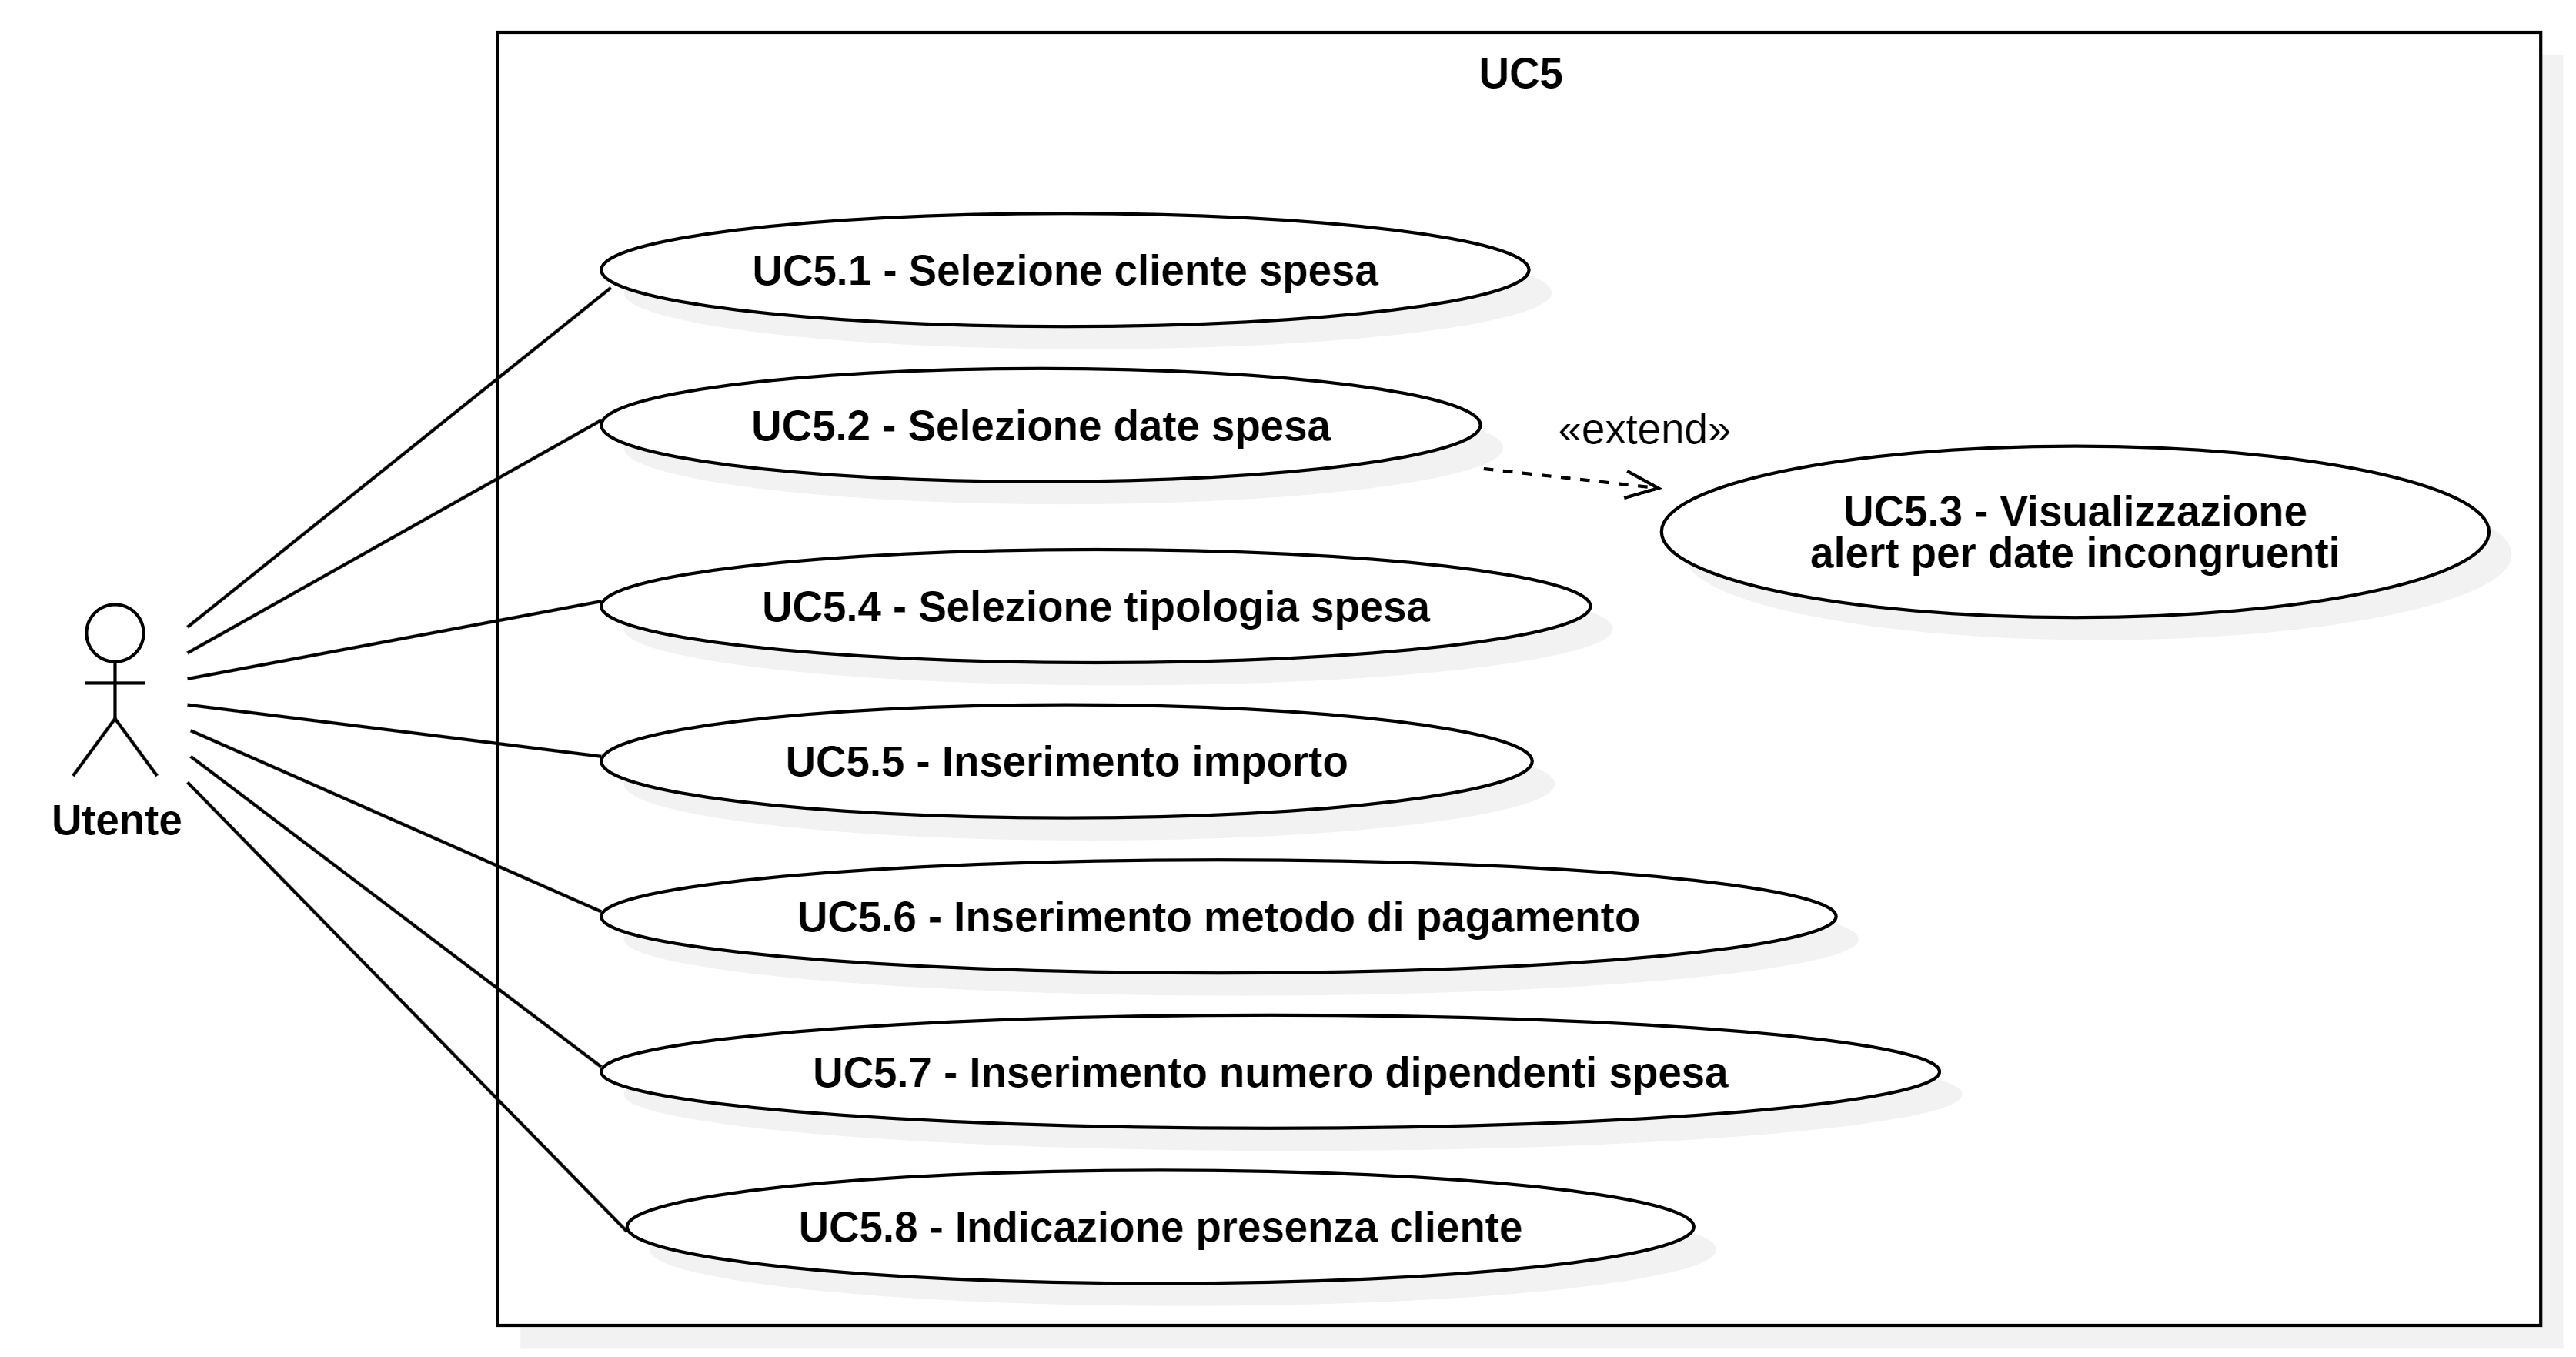
\includegraphics[alt={Use Case 5: Compilazione dati generali spesa}, width=1\columnwidth]{img/usecase/UC5.jpg}
        \caption{UC5: Compilazione dati generali spesa}
        \label{fig:UC5}
    \end{figure}
    \usecaseactors{Utente.}
    \usecasedesc{L'utente compila i campi di input per inserire i dati della spesa.}
    \usecasepre{L'utente ha effettuato l'accesso alla schermata di inserimento di una nuova nota spesa.}
    \usecasepost{I campi della nota spesa vengono valorizzati con i dati inseriti dall'utente.}
    \usecaseprin{
        \begin{itemize}
            \item L'utente seleziona il cliente associato alla spesa (\ref{uc:uc_selezione_cliente_spesa}).
            \item L'utente compila data di inizio e data di fine (\ref{uc:uc_selezione_date_spesa}).
            \item L'utente seleziona la tipologia di spesa (\ref{uc:uc_selezione_tipologia_spesa}).
            \item L'utente compila l'importo (\ref{uc:uc_inserimento_importo_spesa}).
            \item L'utente seleziona il metodo di pagamento (\ref{uc:uc_selezione_metodo_pagamento}).
            \item L'utente indica il numero di dipendenti coinvolti nella spesa (\ref{uc:uc_inserimento_numero_dipendenti_spesa}).
            \item L'utente indica la presenza del cliente (\ref{uc:uc_spunta_presenza_cliente}).
            \item L'utente può inserire le note aggiuntive (\ref{uc:uc_inserimento_note_aggiuntive}).
            \item L'utente allega la foto dello scontrino (\ref{uc:uc_inserimento_foto_scontrino}).
            \item L'utente inserisce il numero documento dello scontrino (\ref{uc:uc_inserimento_nrdoc_scontrino}).
            \item L'utente inserisce la data e l'ora dello scontrino (\ref{uc:uc_inserimento_data_ora_scontrino}).
            \item L'utente inserisce la ragione sociale dello scontrino (\ref{uc:uc_inserimento_ragione_sociale_scontrino}).
            \item L'utente inserisce la partita IVA dello scontrino (\ref{uc:uc_inserimento_partita_iva_scontrino}).
        \end{itemize}
    }
    \label{uc:uc_compilazione_dati_generali_spesa}
\end{usecase}

\begin{usecase}{5.1}{Selezione cliente spesa}
    \usecaseactors{Utente.}
    \usecasedesc{L'utente seleziona il cliente da associare alla spesa.}
    \usecasepre{L'utente è nella schermata di inserimento della nota spesa.}
    \usecasepost{Il sistema registra il cliente associato alla spesa.}
    \usecaseprin{
        \begin{itemize}
            \item L'utente seleziona la voce cliente.
            \item Il sistema mostra la lista dei clienti disponibili.
            \item L'utente ricerca e seleziona un cliente dalla lista.
        \end{itemize}
    }
    \label{uc:uc_selezione_cliente_spesa}
\end{usecase}

\begin{usecase}{5.2}{Selezione date spesa}
    \usecaseactors{Utente.}
    \usecasedesc{L'utente vuole selezionare le date di inizio e di fine della spesa.}
    \usecasepre{L'utente è nella schermata di inserimento della nota spesa.}
    \usecasepost{Il sistema registra le date selezionate.}
    \usecaseprin{
        \begin{itemize}
            \item L'utente seleziona le voci "Da Data" e "A Data".
            \item Il sistema mostra il calendario per la selezione delle date.
            \item L'utente seleziona la data di inizio e la data di fine.
        \end{itemize}
    }
    \label{uc:uc_selezione_date_spesa}
\end{usecase}

\begin{usecase}{5.3}{Visualizzazione alert per date incongruenti}
    \usecaseactors{Utente.}
    \usecasedesc{Il sistema mostra un messaggio di errore se la data di fine spesa è antecedente a quella di inizio.}
    \usecasepre{L'utente in "A data" ha selezionato una data precedente al valore di "Da Data".}
    \usecasepost{L'utente deve reinserire la data.}
    \usecaseprin{
        \begin{itemize}
            \item Il sistema effettua la validazione logica delle date.
            \item Viene mostrato un alert a schermo indicante l'incongruenza.
        \end{itemize}
    }
    \label{uc:uc_errore_date_incongruenti}
\end{usecase}

\begin{usecase}{5.4}{Selezione tipologia di spesa}
    \usecaseactors{Utente.}
    \usecasedesc{L'utente vuole selezionare la tipologia di spesa.}
    \usecasepre{L'utente si trova nella schermata di inserimento.}
    \usecasepost{La tipologia viene valorizzata con la selezione dell'utente. Se viene scelta l'opzione "Altro", il campo "Note" diventa obbligatorio.}
    \usecaseprin{
        \begin{itemize}
            \item L'utente apre il picker della tipologia.
            \item L'utente seleziona una delle 5 opzioni: Pranzo, Cena, Pernottamento, Rifornimento, Altro.
        \end{itemize}
    }
    \label{uc:uc_selezione_tipologia_spesa}
\end{usecase}

\begin{usecase}{5.5}{Inserimento importo}
    \usecaseactors{Utente.}
    \usecasedesc{L'utente vuole inserire l'importo della spesa.}
    \usecasepre{L'utente si trova nella schermata di inserimento.}
    \usecasepost{L'importo viene valorizzato con il valore inserito dall'utente.}
    \usecaseprin{
        \begin{itemize}
            \item L'utente digita l'importo nell'apposita area.
        \end{itemize}
    }
    \label{uc:uc_inserimento_importo_spesa}
\end{usecase}

\begin{usecase}{5.6}{Selezione metodo di pagamento}
    \usecaseactors{Utente.}
    \usecasedesc{L'utente vuole selezionare il metodo di pagamento.}
    \usecasepre{L'utente si trova nella schermata di inserimento.}
    \usecasepost{Il metodo di pagamento viene valorizzato con la selezione dell'utente.}
    \usecaseprin{
        \begin{itemize}
            \item L'utente apre il picker del metodo di pagamento.
            \item L'utente seleziona una delle 3 opzioni: Carta di credito aziendale, Carta di credito personale, Contanti.
        \end{itemize}
    }
    \label{uc:uc_selezione_metodo_pagamento}
\end{usecase}

\begin{usecase}{5.7}{Inserimento numero dipendenti spesa}
    \usecaseactors{Utente.}
    \usecasedesc{L'utente vuole indicare il numero di dipendenti coinvolti nella spesa.}
    \usecasepre{L'utente si trova nella schermata di inserimento.}
    \usecasepost{Il campo viene valorizzato con il valore inserito dall'utente.}
    \usecaseprin{
        \begin{itemize}
            \item L'utente digita il numero di dipendenti nell'apposita area o utilizza i bottoni di incremento/decremento.
        \end{itemize}
    }
    \label{uc:uc_inserimento_numero_dipendenti_spesa}
\end{usecase}

\begin{usecase}{5.8}{Indicazione presenza cliente}
    \usecaseactors{Utente.}
    \usecasedesc{L'utente vuole indicare la presenza di uno o più rappresentanti del cliente nella spesa.}
    \usecasepre{L'utente si trova nella schermata di inserimento.}
    \usecasepost{La casella viene spuntata o deselezionata.}
    \usecaseprin{
        \begin{itemize}
            \item L'utente spunta o deseleziona l'apposita casella.
        \end{itemize}
    }
    \label{uc:uc_spunta_presenza_cliente}
\end{usecase}

\begin{usecase}{6}{Inserimento note aggiuntive}
    \usecaseactors{Utente.}
    \usecasedesc{L'utente vuole inserire una descrizione o causale testuale. Questo campo diviene obbligatorio se la tipologia selezionata è "Altro".}
    \usecasepre{L'utente si trova nella schermata di inserimento.}
    \usecasepost{Il campo di testo delle note viene valorizzato.}
    \usecaseprin{
        \begin{itemize}
            \item L'utente digita il testo nell'apposita area.
        \end{itemize}
    }
    \label{uc:uc_inserimento_note_aggiuntive}
\end{usecase}

\begin{figure}[H]
    \vspace{2em}
    \centering
    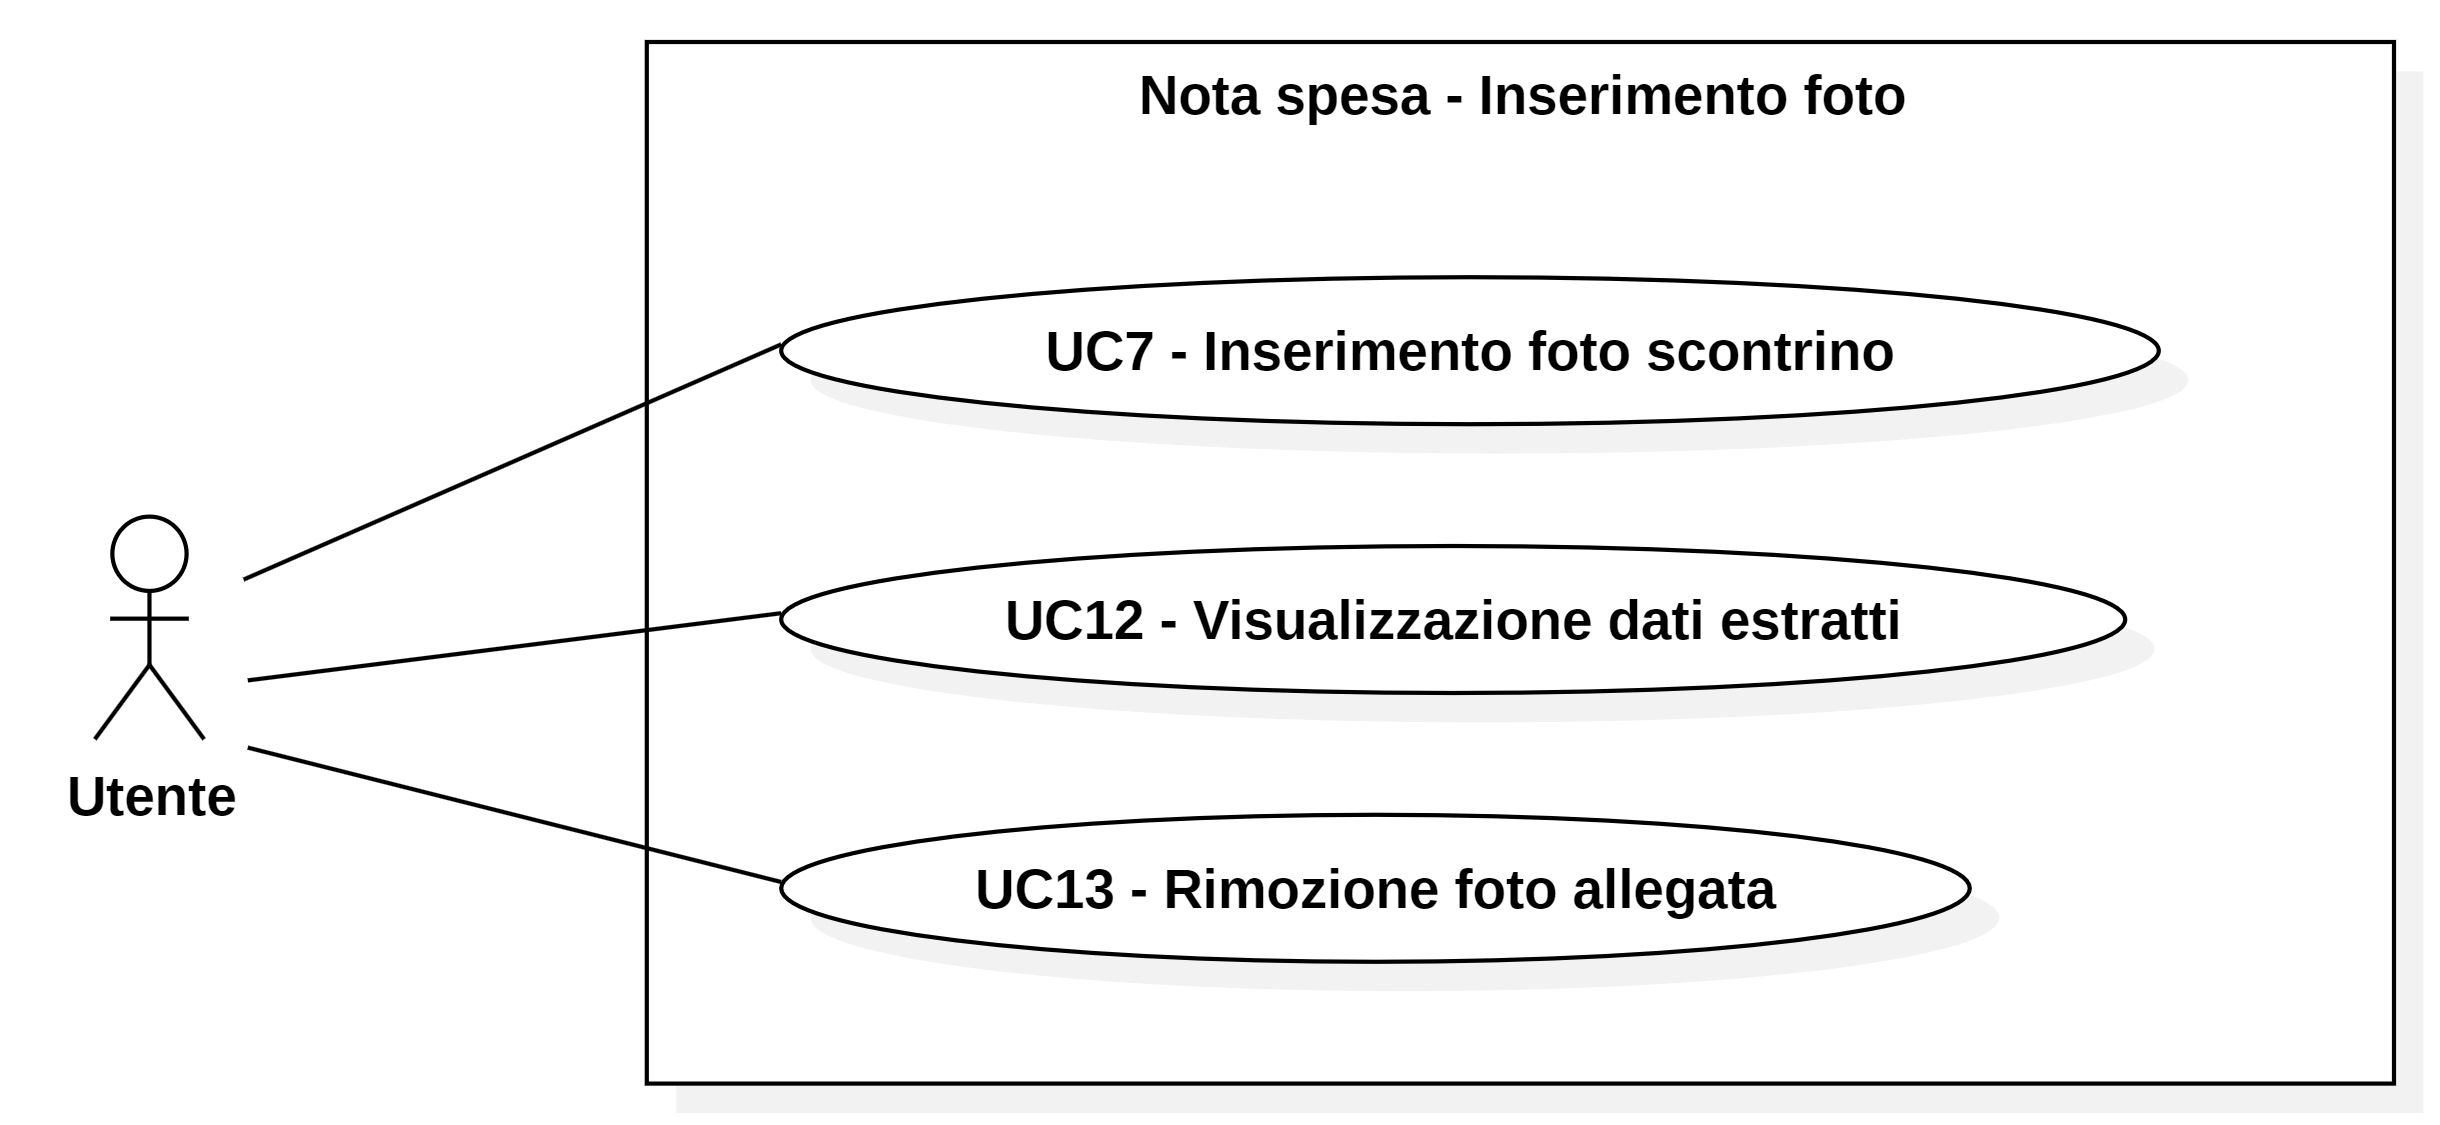
\includegraphics[alt={Scenario di inserimento della foto}, width=0.85\columnwidth]{img/usecase/UCFoto.jpg}
    \caption{Nota spesa: Inserimento foto}
    \label{fig:UCFoto}
\end{figure}

\begin{usecase}{7}{Inserimento foto scontrino}
    \begin{figure}[H]
        \vspace{2em}
        \centering
        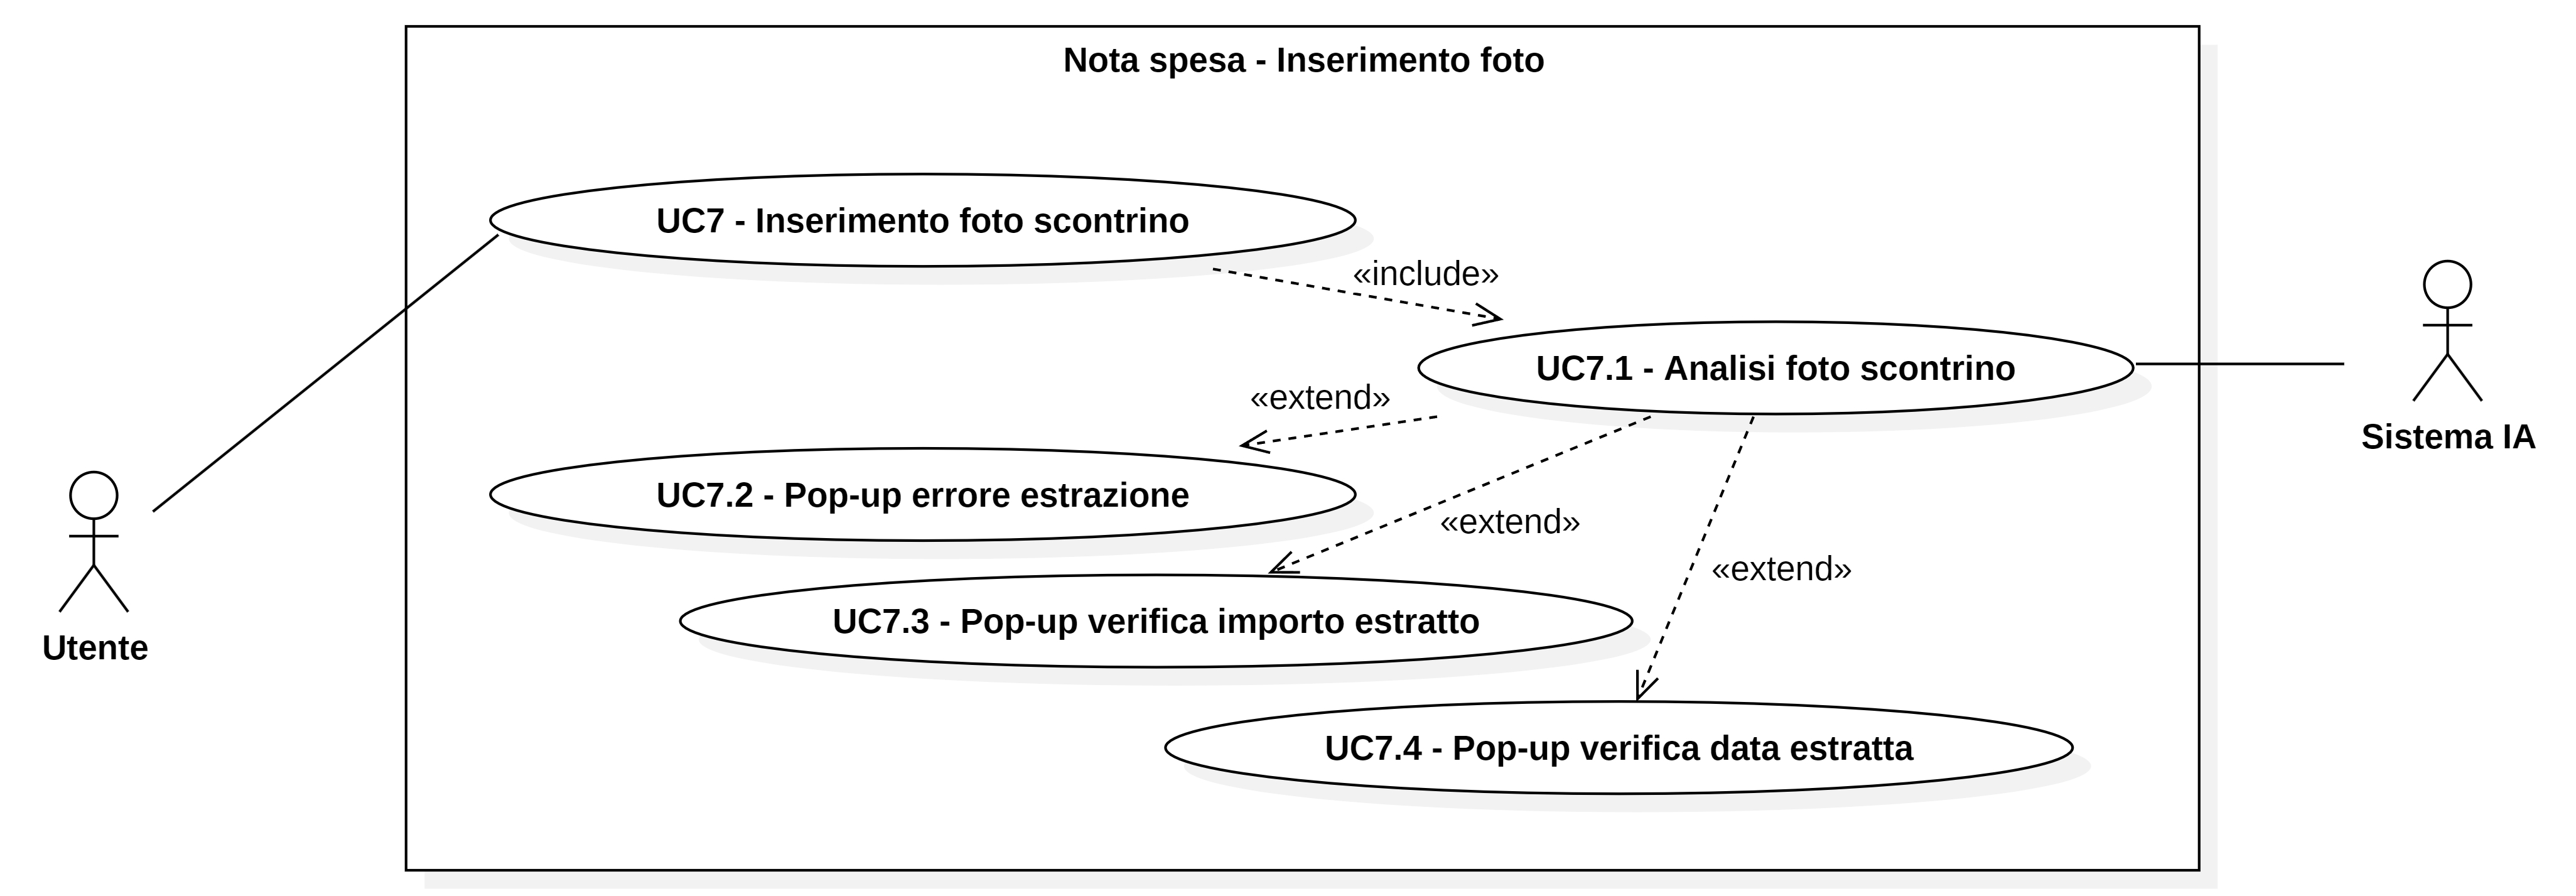
\includegraphics[alt={Use Case 7: Inserimento foto scontrino}, width=1\columnwidth]{img/usecase/UC7.jpg}
        \caption{UC7: Inserimento foto scontrino}
        \label{fig:UC7}
    \end{figure}
    \usecaseactors{Utente.}
    \usecasedesc{L'utente inserisce una foto dello scontrino.}
    \usecasepre{L'utente è nella schermata di inserimento della nota spesa e ha selezionato la funzionalità di inserimento foto scontrino.}
    \usecasepost{Il sistema registra l'immagine allegata.}
    \usecaseprin{
        \begin{itemize}
            \item L'utente seleziona l'opzione per allegare la foto dello scontrino.
            \item L'utente scatta una foto o seleziona un'immagine dalla galleria del dispositivo.
        \end{itemize}
    }
    \label{uc:uc_inserimento_foto_scontrino}
\end{usecase}

\begin{usecase}{7.1}{Analisi foto scontrino}
    \usecaseactors{Sistema \gls{ia}.}
    \usecasedesc{Il sistema analizza la foto dello scontrino per estrarre i dati.}
    \usecasepre{L'utente ha inserito una foto dello scontrino.}
    \usecasepost{Il sistema registra i dati estratti dalla foto.}
    \usecaseprin{
        \begin{itemize}
            \item Il sistema analizza l'immagine per identificare i dati.
            \item Il sistema estrae informazioni come data, ora, importo, numero documento, ragione sociale e partita iva dalla foto allegata.
        \end{itemize}
    }
    \label{uc:uc_analisi_foto_scontrino}
\end{usecase}

\begin{usecase}{7.2}{Pop-up errore estrazione}
    \usecaseactors{Utente, Sistema \gls{ia}.}
    \usecasedesc{Il sistema mostra un messaggio di errore}
    \usecasepre{L'utente ha inserito una foto e il sistema IA ha avviato l'analisi.}
    \usecasepost{Il sistema mostra un messaggio di errore.}
    \usecaseprin{
        \begin{itemize}
            \item La connessione è assente oppure il sistema \gls{ia} non riesce ad estrarre alcun dato dalla foto allegata.
            \item L'utente visualizza un messaggio di errore.
        \end{itemize}
    }
    \label{uc:uc_pop-up_errore_estrazione}
\end{usecase}

\begin{usecase}{7.3}{Pop-up verifica importo estratto}
    \usecaseactors{Utente.}
    \usecasedesc{L'utente verifica l'importo estratto dalla foto allegata.}
    \usecasepre{L'utente ha precedentemente inserito un importo e successivamente ha inserito una foto.}
    \usecasepost{Il sistema memorizza l'importo scelto dall'utente.}
    \usecaseprin{
        \begin{itemize}
            \item Il sistema mostra un pop-up per comunicare all'utente che l'importo estratto dalla foto è differente da quello digitato manualmente.
            \item L'utente sceglie se mantenere l'importo digitato o se sostituirlo con quello estratto.
        \end{itemize}
    }
    \label{uc:uc_pop-up_verifica_importo_estratto}
\end{usecase}

\begin{usecase}{7.4}{Pop-up verifica data estratta}
    \usecaseactors{Utente.}
    \usecasedesc{L'utente verifica la data estratta dalla foto allegata.}
    \usecasepre{L'utente ha inserito una foto.}
    \usecasepost{Il sistema memorizza la data scelta dall'utente.}
    \usecaseprin{
        \begin{itemize}
            \item Il sistema mostra un pop-up per comunicare all'utente che la data estratta dalla foto è minore della data minima consentita dal sistema.
            \item L'utente sceglie se mantenere la data attuale o se sostituirla con quella estratta.
        \end{itemize}
    }
    \label{uc:uc_pop-up_verifica_data_estratta}
\end{usecase}

\begin{usecase}{8}{Inserimento numero documento scontrino}
    \usecaseactors{Utente.}
    \usecasedesc{L'utente vuole inserire o modificare il numero del documento dello scontrino.}
    \usecasepre{L'utente si trova nella schermata di inserimento e ha allegato una foto dello scontrino.}
    \usecasepost{Il campo viene valorizzato con il valore inserito dall'utente.}
    \usecaseprin{
        \begin{itemize}
            \item L'utente digita il testo nell'apposita area.
        \end{itemize}
    }
    \label{uc:uc_inserimento_nrdoc_scontrino}
\end{usecase}

\begin{usecase}{9}{Inserimento data e ora scontrino}
    \usecaseactors{Utente.}
    \usecasedesc{L'utente vuole inserire o modificare la data e l'ora dello scontrino.}
    \usecasepre{L'utente si trova nella schermata di inserimento e ha allegato una foto dello scontrino.}
    \usecasepost{Il campo viene valorizzato con il valore inserito dall'utente.}
    \usecaseprin{
        \begin{itemize}
            \item L'utente digita il testo nell'apposita area.
        \end{itemize}
    }
    \label{uc:uc_inserimento_data_ora_scontrino}
\end{usecase}

\begin{usecase}{10}{Inserimento ragione sociale scontrino}
    \usecaseactors{Utente.}
    \usecasedesc{L'utente vuole inserire o modificare la ragione sociale dello scontrino.}
    \usecasepre{L'utente si trova nella schermata di inserimento e ha allegato una foto dello scontrino.}
    \usecasepost{Il campo viene valorizzato con il valore inserito dall'utente.}
    \usecaseprin{
        \begin{itemize}
            \item L'utente digita il testo nell'apposita area.
        \end{itemize}
    }
    \label{uc:uc_inserimento_ragione_sociale_scontrino}
\end{usecase}

\begin{usecase}{11}{Inserimento partita iva scontrino}
    \usecaseactors{Utente.}
    \usecasedesc{L'utente vuole inserire o modificare la partita iva dello scontrino.}
    \usecasepre{L'utente si trova nella schermata di inserimento e ha allegato una foto dello scontrino.}
    \usecasepost{Il campo viene valorizzato con il valore inserito dall'utente.}
    \usecaseprin{
        \begin{itemize}
            \item L'utente digita il testo nell'apposita area.
        \end{itemize}
    }
    \label{uc:uc_inserimento_partita_iva_scontrino}
\end{usecase}

\begin{usecase}{12}{Visualizzazione dati estratti}
    \usecaseactors{Utente, Sistema \gls{ia}.}
    \usecasedesc{L'utente visualizza i dati estratti dalla foto dello scontrino.}
    \usecasepre{L'utente ha inserito una foto e il sistema ha estratto correttamente i dati da essa.}
    \usecasepost{Il sistema mostra i dati estratti dalla foto.}
    \usecaseprin{
        \begin{itemize}
            \item L'utente visualizza i dati estratti.
        \end{itemize}
    }
    \label{uc:uc_visualizzazione_dati_estratti}
\end{usecase}

\begin{usecase}{13}{Rimozione foto allegata}
    \usecaseactors{Utente.}
    \usecasedesc{L'utente vuole rimuovere una foto precedentemente caricata.}
    \usecasepre{Un'immagine è stata allegata ed eventuali dati estratti sono visibili.}
    \usecasepost{Il sistema elimina la foto dalla memoria, resetta i valori estratti e nasconde i relativi campi dalla schermata.}
    \usecaseprin{
        \begin{itemize}
            \item L'utente utilizza la funzionalità per rimuovere la foto.
        \end{itemize}
    }
    \label{uc:uc_rimozione_foto_allegata}
\end{usecase}

\begin{figure}[H]
    \vspace{2em}
    \centering
    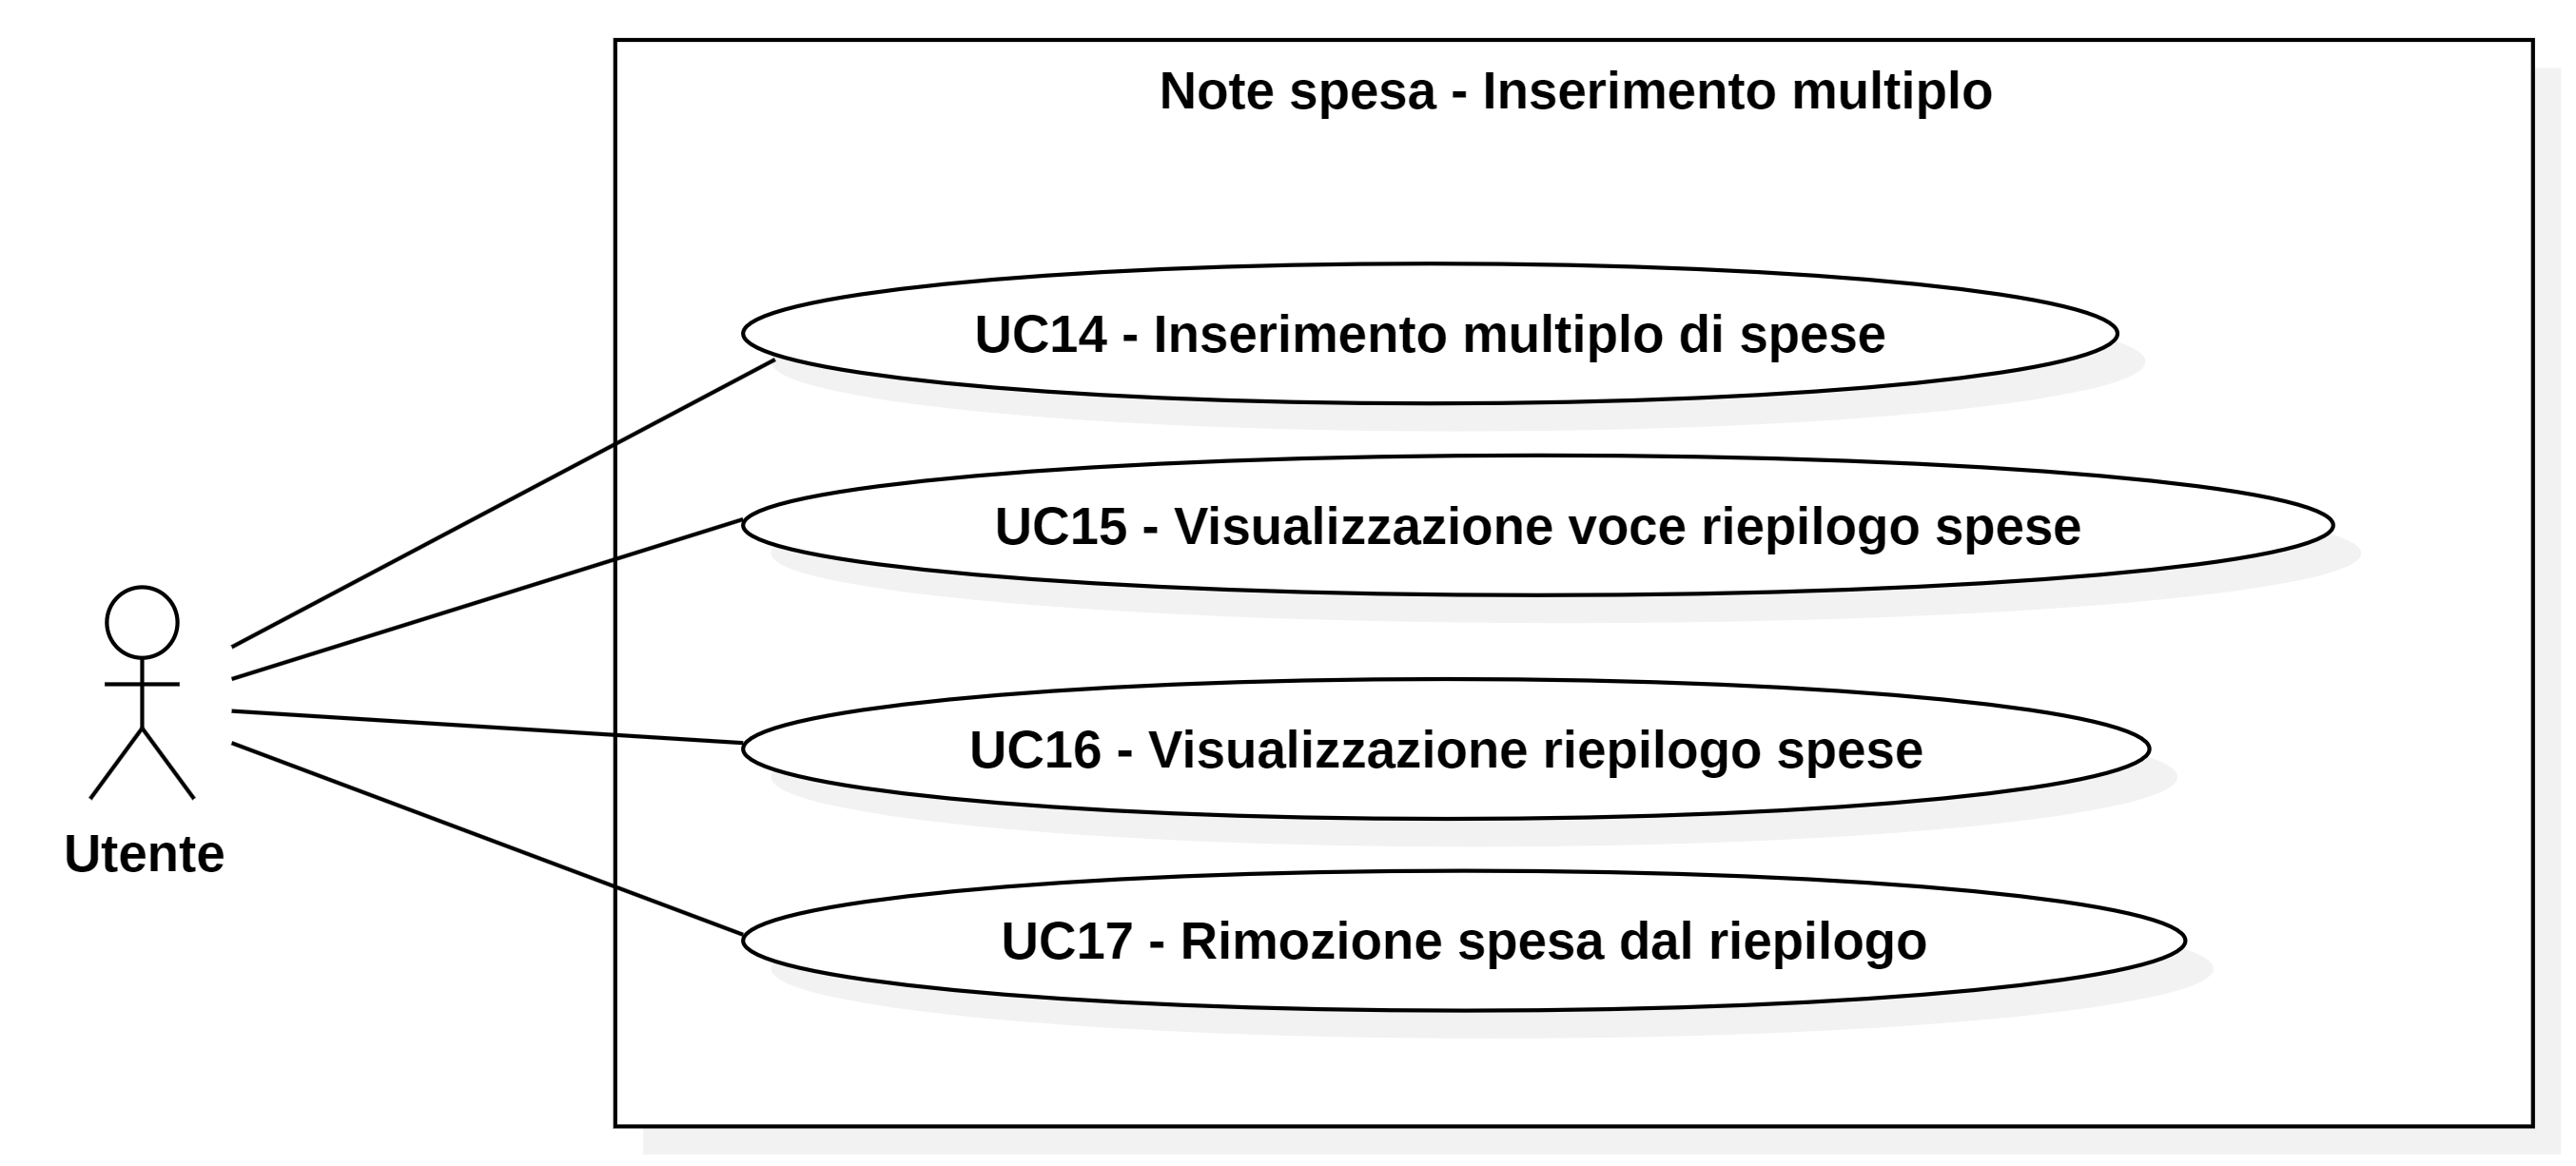
\includegraphics[alt={Scenario di inserimento multiplo in una nota spesa}, width=0.84\columnwidth]{img/usecase/UCMultiplo.jpg}
    \caption{Nota spesa: Inserimento multiplo}
    \label{fig:UCMultiplo}
\end{figure}

\begin{usecase}{14}{Inserimento multiplo di spese}
    \usecaseactors{Utente.}
    \usecasedesc{L'utente preme il pulsante "AGGIUNGI UN'ALTRA SPESA" per inserire un'ulteriore transazione all'interno della medesima nota spesa.}
    \usecasepre{L'utente ha compilato correttamente i dati di una prima spesa e ha valorizzato il campo Cliente.}
    \usecasepost{La modifica al campo Cliente viene disabilitata e vengono  portati ai valori di default i restanti campi del from.}
    \usecaseprin{
        \begin{itemize}
            \item L'utente preme il bottone "AGGIUNGI UN'ALTRA SPESA".
            \item Il sistema salva temporaneamente in memoria la spesa appena compilata.
        \end{itemize}
    }
    \label{uc:uc_aggiungi_altra_spesa}
\end{usecase}

\begin{usecase}{15}{Visualizzazione voce riepilogo spese}
    \usecaseactors{Utente.}
    \usecasedesc{L'utente visualizza una voce dedicata al riepilogo delle spese salvate temporaneamente tramite la funzionalità di inserimento multiplo.}
    \usecasepre{L'utente ha utilizzato almento una volta la funzionalità di inserimento multiplo (\ref{uc:uc_aggiungi_altra_spesa}).}
    \usecasepost{Il sistema mostra una voce integrata nell'interfaccia, sotto il campo cliente.}
    \usecaseprin{
        \begin{itemize}
            \item L'utente visualizza la voce "Riepilogo spese inserite" posta sotto il campo cliente.
            \item L'utente può espandere la voce per visualizzare l'elenco delle spese già inserite.
        \end{itemize}
    }
    \label{uc:uc_visualizzazione_voce_riepilogo_spese}
\end{usecase}

\begin{usecase}{16}{Visualizzazione riepilogo spese}
    \usecaseactors{Utente.}
    \usecasedesc{L'utente espande la sezione dedicata per visualizzare l'elenco delle spese salvate temporaneamente tramite la funzionalità di inserimento multiplo.}
    \usecasepre{L'utente ha cliccato sulla voce "Riepilogo spese inserite".}
    \usecasepost{L'utente visualizza i dettagli delle spese inserite.}
    \usecaseprin{
        \begin{itemize}
            \item Il sistema espande la sezione "Riepilogo spese inserite" nell'interfaccia corrente.
            \item Per ogni spesa inserita vengono mostrati: tipologia, data, importo e un'icona a forma di cestino per rimuovere la spesa.
        \end{itemize}
    }
    \label{uc:uc_visualizzazione_riepilogo_spese}
\end{usecase}

\begin{usecase}{17}{Rimozione spesa dal riepilogo}
    \usecaseactors{Utente.}
    \usecasedesc{L'utente vuole rimuovere una spesa dal riepilogo delle spese inserite temporaneamente.}
    \usecasepre{L'utente ha cliccato sulla voce "Riepilogo spese inserite" e visualizza il riepilogo.}
    \usecasepost{La spesa viene rimossa dal riepilogo e dal sistema.}
    \usecaseprin{
        \begin{itemize}
            \item L'utente preme sull'icona a forma di cestino accanto alla spesa che desidera rimuovere.
            \item Il sistema mostra un pop-up di conferma.
            \item L'utente conferma la rimozione.
        \end{itemize}
    }
    \usecasealt{
        \begin{itemize}
            \item L'utente seleziona "ANNULLA".
            \item Il sisteam chiude il pop-up senza eliminare la spesa.
        \end{itemize}
    }
    \label{uc:uc_rimozione_spesa_riepilogo}
\end{usecase}

\begin{usecase}{18}{Pop-up promemoria sincronizzazione}
    \usecaseactors{Utente.}
    \usecasedesc{Il sistema mostra un pop-up per ricordare all'utente di sincronizzare le note spesa locali.}
    \usecasepre{L'utente ha effettuato l'accesso all'applicazione e ha navigato nella sezione dedicata alle note spesa per la prima volta da quando ha aperto l'applicazione. È presente almeno una nota spesa locale non sincronizzata.}
    \usecasepost{Il sistema registra la risposta dell'utente}
    \usecaseprin{
        \begin{itemize}
            \item Il sistema mostra il pop-up di promemoria.
            \item Il pop-up chiede all'utente se vuole procedere con la sincronizzazione delle note spesa locali, mostrando i pulsanti "ANNULLA" e "SINCRONIZZA ORA" (\ref{uc:uc_sincronizzazione_note}).
        \end{itemize}
    }
    \label{uc:uc_pop-up_promemoria_sincronizzazione}
\end{usecase}

\begin{usecase}{19}{Visualizzazione dettaglio mensile}
    \usecaseactors{Utente.}
    \usecasedesc{L'utente visualizza la lista di tutte le note spesa appartenenti a uno specifico resoconto mensile.}
    \usecasepre{L'utente ha selezionato un resoconto mensile dalla schermata principale (\ref{uc:uc_visualizzazione_singolo_resoconto}).}
    \usecasepost{Il sistema mostra l'elenco delle note spesa contenute nel mese selezionato.}
    \usecaseprin{
        \begin{itemize}
            \item Il sistema effettua il caricamento dei dati relativi al mese scelto.
            \item L'utente visualizza l'elenco delle note spesa con data, tipologia, cliente e importo.
            \item L'utente può visualizzare un'eventuale icona di stato per le note non sincronizzate.
        \end{itemize}
    }
    \label{uc:uc_visualizzazione_dettaglio_mensile}
\end{usecase}

\begin{figure}[H]
    \vspace{2em}
    \centering
    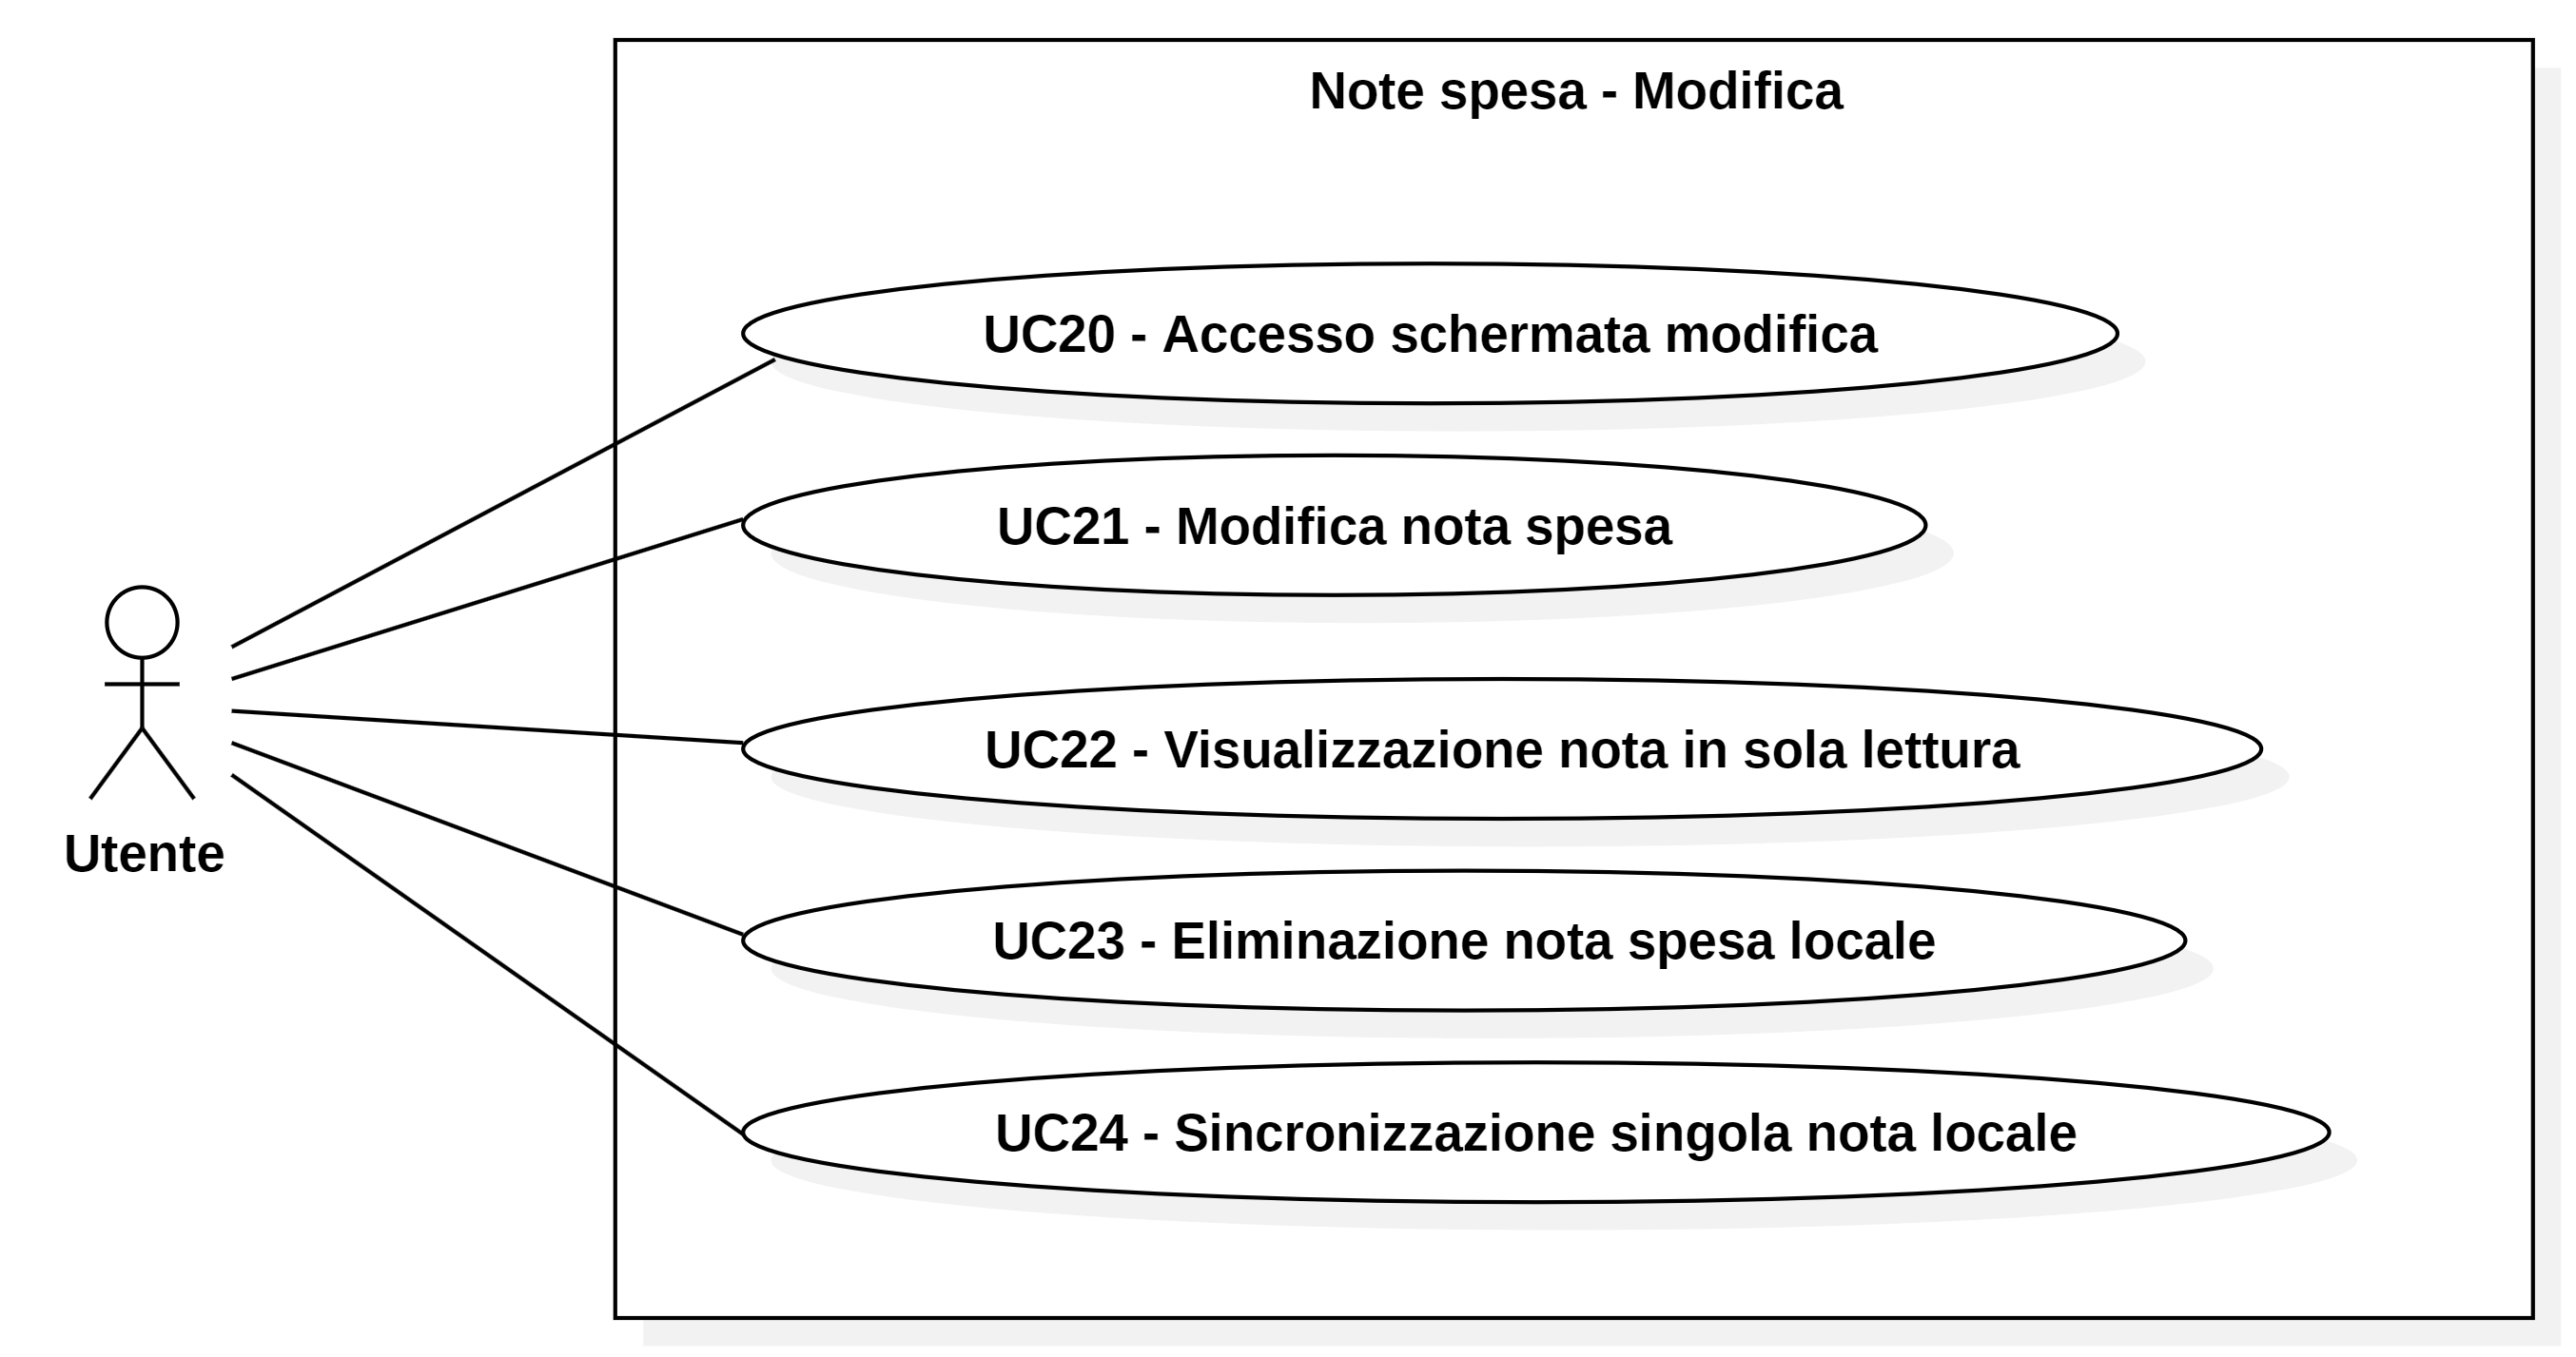
\includegraphics[alt={Scenario di modifica di una nota spesa}, width=0.90\columnwidth]{img/usecase/UCModifica.jpg}
    \caption{Nota spesa: Modifica nota}
    \label{fig:UCModifica}
\end{figure}

\begin{usecase}{20}{Accesso schermata modifica}
    \usecaseactors{Utente.}
    \usecasedesc{L'utente vuole accedere alla schermata di modifica di una nota spesa.}
    \usecasepre{L'utente si trova nella schermata di dettaglio mensile.}
    \usecasepost{La nota spesa viene caricata e tutti i campi vengono precompilati.}
    \usecaseprin{
        \begin{itemize}
            \item L'utente preme su una delle note spesa della lista.
            \item Il sistema recupera i dati completi della nota spesa.
            \item Il sistema carica la schermata di inserimento, popolando i campi con i valori della nota selezionata.
        \end{itemize}
    }
    \label{uc:uc_accesso_modifica_nota}
\end{usecase}

\begin{usecase}{21}{Modifica nota spesa}
    \usecaseactors{Utente.}
    \usecasedesc{L'utente modifica i dati di una nota spesa precedentemente salvata.}
    \usecasepre{L'utente ha effettuato l'accesso alla schermata di modifica di una nota (\ref{uc:uc_accesso_modifica_nota}).}
    \usecasepost{La nota viene aggiornata e l'utente reindirizzato alla schermata precedente.}
    \usecaseprin{
        \begin{itemize}
            \item Il sistema mostra il form con i campi precompilati.
            \item L'utente modifica uno o più campi della nota spesa.
            \item L'utente conferma le modifiche.
            \item Il sistema aggiorna la nota sul server.
        \end{itemize}
    }
    \usecasealt{
        \begin{itemize}
            \item Il dispositivo non dispone di una connessione a Internet.
            \item Il sistema salva le modifiche nel database locale.
            \item Il sistema contrassegna la nota con stato "locale".
        \end{itemize}
    }
    \label{uc:uc_modifica_nota_spesa}
\end{usecase}

\begin{usecase}{22}{Visualizzazione nota in sola lettura}
    \usecaseactors{Utente.}
    \usecasedesc{Il sistema disabilita la modifica di tutti i campi del form se la nota spesa caricata fa riferimento a una data storicizzata (precedente alla data minima consentita).}
    \usecasepre{L'utente si trova nella schermata di dettaglio mensile e ha selezionato una nota spesa per modificarla. La data della nota è antecedente al limite consentito.}
    \usecasepost{L'utente visualizza i dati senza poterli alterare.}
    \usecaseprin{
        \begin{itemize}
            \item Il sistema effettua un controllo logico sulla data della nota.
            \item Il sistema rende in sola lettura tutti i campi di input.
            \item Vengono nascosti eventuali pulsanti di salvataggio.
        \end{itemize}
    }
    \label{uc:uc_nota_sola_lettura}
\end{usecase}

\begin{usecase}{23}{Eliminazione nota spesa locale}
    \usecaseactors{Utente.}
    \usecasedesc{L'utente vuole eliminare definitivamente una nota spesa salvata localmente.}
    \usecasepre{L'utente si trova in modalità modifica di una nota con stato "locale".}
    \usecasepost{La nota viene rimossa dal database locale del dispositivo.}
    \usecaseprin{
        \begin{itemize}
            \item L'utente preme il pulsante per l'eliminazione.
            \item Il sistema mostra un pop-up di conferma.
            \item L'utente seleziona "SI".
            \item Il sistema elimina la nota dal database locale.
        \end{itemize}
    }
    \usecasealt{
        \begin{itemize}
            \item L'utente seleziona "ANNULLA".
            \item Il sistema chiude il pop-up senza eliminare la nota.
        \end{itemize}
    }
    \label{uc:uc_eliminazione_nota_locale}
\end{usecase}

\begin{usecase}{24}{Sincronizzazione singola nota locale}
    \usecaseactors{Utente.}
    \usecasedesc{L'utente vuole sincronizzare immediatamente una nota spesa salvata localmente.}
    \usecasepre{L'utente si trova in modalità modifica di una nota con stato "locale" e dispone di connessione a Internet.}
    \usecasepost{La nota viene inviata al server e assume lo stato "sincronizzata".}
    \usecaseprin{
        \begin{itemize}
            \item L'utente preme il pulsante di caricamento.
            \item Il sistema invia la nota al server e sincronizza il database locale.
        \end{itemize}
    }
    \usecasealt{
        \begin{itemize}
            \item La sincronizzazione fallisce.
            \item Il sistema mantiene la nota nello stato "locale".
            \item Il sistema mostra un messaggio di errore.
        \end{itemize}
    }
    \label{uc:uc_sincronizzazione_nota_locale}
\end{usecase}



\section{Tracciamento dei requisiti}
\noindent A seguito dell'analisi preliminare e della stesura dei casi d'uso, è stato possibile redigere un elenco completo dei requisiti del sistema. Questo processo è fondamentale per garantire che ogni funzionalità implementata risponda a una specifica necessità del committente e per facilitare le successive fasi di validazione e collaudo. \\
Per classificare i requisiti in modo univoco e strutturato, è stata adottata la seguente codifica alfanumerica:
\begin{center}
    \textbf{R[Tipologia][Importanza]-[Numero progressivo]}
\end{center}
\noindent La \textbf{Tipologia} del requisito può assumere i seguenti valori:
\begin{itemize}
    \item \textbf{F (Funzionale):} descrive le funzioni e i comportamenti che il sistema deve offrire all'utente;
    \item \textbf{Q (Qualitativo):} definisce gli standard di qualità, usabilità e manutenibilità del codice;
    \item \textbf{V (Di Vincolo):} impone restrizioni tecnologiche o architetturali, spesso dettate dall'ambiente aziendale preesistente.
\end{itemize}

\noindent L'\textbf{Importanza} del requisito è classificata come segue:
\begin{itemize}
    \item \textbf{O (Obbligatorio):} funzionalità vitale, la cui mancanza compromette l'intero progetto;
    \item \textbf{D (Desiderabile):} funzionalità non strettamente necessaria ma dal forte valore aggiunto;
    \item \textbf{F (Facoltativo):} funzionalità secondaria, da implementare solo in caso di tempo residuo.
\end{itemize}

\noindent Nelle tabelle \ref{tab:requisiti_funzionali}, \ref{tab:requisiti_qualitativi} e \ref{tab:requisiti_vincolo} sono riassunti i requisiti e il loro tracciamento con gli use case delineati in fase di analisi.

\section{Tabelle dei requisiti}
\begin{center}
    \rowcolors{1}{}{tableGray}
    \begin{longtable}{|p{2.15cm}|p{7.75cm}|p{2.35cm}|}
    \hline
    \multicolumn{1}{|c|}{\textbf{Requisito}} & \multicolumn{1}{c|}{\textbf{Descrizione}} & \multicolumn{1}{c|}{\textbf{Use Case}}\\
    \hline 
    \endfirsthead
    \rowcolor{white}
    \multicolumn{3}{c}{{\bfseries \tablename\ \thetable{} -- Continuo della tabella}}\\
    \hline
    \multicolumn{1}{|c|}{\textbf{Requisito}} & \multicolumn{1}{c|}{\textbf{Descrizione}} & \multicolumn{1}{c|}{\textbf{Use Case}}\\
    \hline 
    \endhead
    \hline
    \rowcolor{white}
    \multicolumn{3}{|r|}{{Continua nella prossima pagina...}}\\
    \hline
    \endfoot
    \endlastfoot
    RFO-1 & L'utente deve poter visualizzare la lista dei resoconti mensili delle proprie note spesa. & UC1, UC1.1 \\ \hline
    RFO-2 & L'utente deve poter filtrare i resoconti mensili in base all'anno desiderato. & UC2 \\ \hline
    RFO-3 & L'utente deve poter inserire una nuova nota spesa. & UC4, UC5 \\ \hline
    RFO-4 & Il sistema deve validare i dati inseriti e impedire il salvataggio in caso di informazioni mancanti o errate. & UC4.4, UC5.3 \\ \hline
    RFO-5 &  L'utente deve poter inserire una descrizione per ogni spesa. & UC6 \\ \hline
    RFO-6 & L'utente deve poter allegare una fotografia dello scontrino per estrarne automaticamente i dati tramite \gls{ia}. & UC7, UC7.1 \\ \hline
    RFO-7 & L'utente deve poter visualizzare e modificare i dati estratti tramite \gls{ia}. & UC8, UC9, UC10, UC11, UC12 \\ \hline
    RFO-8 & L'utente deve poter rimuovere una foto precedentemente allegata. & UC13 \\ \hline
    RFO-9 & L'utente deve poter aggiungere e accodare transazioni multiple all'interno di un singolo inserimento di nota spesa. & UC14, UC15, UC16 \\ \hline
    RFO-10 & Il sistema deve gestire il salvataggio locale (offline) delle note in caso di assenza di rete o di scelta volontaria. & UC4.2, UC4.4 \\ \hline
    RFO-11 & L'utente deve poter sincronizzare in blocco o singolarmente le note salvate in locale. & UC3, UC24 \\ \hline
    RFO-12 & L'utente deve poter visualizzare le note spesa appartenenti a un singolo resoconto mensile & UC19 \\ \hline
    RFO-13 & L'utente deve poter eliminare una nota spesa esistente, purché non sia storicizzata. & UC23 \\ \hline
    RFO-14 & Il sistema deve impedire la modifica delle note spesa antecedenti alla data minima consentita. & UC22 \\ \hline
    
    RFD-1 & Il sistema deve gestire i conflitti tra i dati inseriti manualmente e quelli estratti dall'\gls{ia} tramite pop-up. & UC7.2, UC7.3, UC7.4 \\ \hline
    RFD-2 & L'utente deve poter rimuovere una spesa salvata temporaneamente tramite inserimento multiplo. & UC17 \\ \hline
    RFD-3 & Il sistema deve ricordare all'utente, all'avvio del modulo, la presenza di note locali non sincronizzate. & UC18 \\ \hline
    RFD-4 & L'utente deve poter accedere alla modalità modifica di una nota spesa. & UC20 \\ \hline
    RFD-5 &  L'utente deve poter modificare una nota spesa esistente. & UC21 \\ \hline
    RFD-6 & L'utente deve poter visualizzare i dati relativi alle proprie note spesa all'interno delle dashboard aziendali preesistenti & TODO \\
    \hline
    \hline
    \hiderowcolors
    \caption{Tabella del tracciamento dei requisiti funzionali.}
    \label{tab:requisiti_funzionali}
    \end{longtable}
\end{center}

\begin{center}
    \rowcolors{1}{}{tableGray}
    \begin{longtable}{|p{2.15cm}|p{7.75cm}|p{2.35cm}|}
    \hline
    \multicolumn{1}{|c|}{\textbf{Requisito}} & \multicolumn{1}{c|}{\textbf{Descrizione}} & \multicolumn{1}{c|}{\textbf{Use Case}}\\
    \hline 
    \endfirsthead
    \rowcolor{white}
    \multicolumn{3}{c}{{\bfseries \tablename\ \thetable{} -- Continuo della tabella}}\\
    \hline
    \multicolumn{1}{|c|}{\textbf{Requisito}} & \multicolumn{1}{c|}{\textbf{Descrizione}} & \multicolumn{1}{c|}{\textbf{Use Case}}\\
    \hline 
    \endhead
    \hline
    \rowcolor{white}
    \multicolumn{3}{|r|}{{Continua nella prossima pagina...}}\\
    \hline
    \endfoot
    \endlastfoot
    
    RQO-1 & L'interfaccia utente deve comunicare chiaramente lo stato delle operazioni tramite messaggi bloccanti o temporanei. & - \\ \hline
    RQO-2 & L'architettura del codice \textit{frontend} deve rispettare rigorosamente il pattern architetturale \gls{mvvm} per separare logica e UI. & - \\ \hline
    RQO-3 & È necessario realizzare opportuni test di accettazione per validare le funzionalità dell'applicazione. & - \\ \hline
    RQO-4 & È necessario realizzare un manuale utente per l'utilizzo dell'applicazione. & - \\ \hline
    RQD-1 & Il codice prodotto deve essere adeguatamente commentato per favorirne la manutenzione da parte di altri sviluppatori Ergon. & - \\ \hline
    \hiderowcolors
    \caption{Tabella del tracciamento dei requisiti qualitativi.}
    \label{tab:requisiti_qualitativi}
    \end{longtable}
\end{center}

\begin{center}
    \rowcolors{1}{}{tableGray}
    \begin{longtable}{|p{2.15cm}|p{7.75cm}|p{2.35cm}|}
    \hline
    \multicolumn{1}{|c|}{\textbf{Requisito}} & \multicolumn{1}{c|}{\textbf{Descrizione}} & \multicolumn{1}{c|}{\textbf{Use Case}}\\
    \hline 
    \endfirsthead
    \rowcolor{white}
    \multicolumn{3}{c}{{\bfseries \tablename\ \thetable{} -- Continuo della tabella}}\\
    \hline
    \multicolumn{1}{|c|}{\textbf{Requisito}} & \multicolumn{1}{c|}{\textbf{Descrizione}} & \multicolumn{1}{c|}{\textbf{Use Case}}\\
    \hline 
    \endhead
    \hline
    \rowcolor{white}
    \multicolumn{3}{|r|}{{Continua nella prossima pagina...}}\\
    \hline
    \endfoot
    \hline
    \hiderowcolors
    \caption{Tabella del tracciamento dei requisiti di vincolo.}
    \label{tab:requisiti_vincolo}
    \endlastfoot
    
    RVO-1 & Il software prodotto deve essere sviluppato in \gls{csharpg} utilizzando il framework \textit{cross-platform} \gls{dotnetmauig}. & - \\ \hline
    RVO-2 & L'interfaccia grafica deve essere realizzata tramite linguaggio di markup \gls{xamlg}, integrandosi nel design system dell'app \gls{ergteam}. & - \\ \hline
    RVO-3 & Il modulo \textit{backend} deve essere implementato aggiungendo i nuovi endpoint REST. & - \\ \hline
    RVO-4 & L'applicazione deve funzionare su dispositivi Android. & - \\ \hline
    RVO-5 & L'applicazione deve funzionare su dispositivi iOS. & - \\ \hline
    RVO-6 & I dati delle note spesa inviati al \textit{backend} devono integrarsi con l'\gls{erp} aziendale per la gestione amministrativa. & - \\ \hline
    RVO-7 & Per il servizio di estrazione dati dalle immagini deve essere interrogata l'\gls{api} di Azure Content Understanding. & - \\
    \hiderowcolors
    \end{longtable}
\end{center}

\begin{center}
    \rowcolors{1}{}{tableGray}
    \begin{longtable}{|p{3.25cm}|p{3.00cm}|p{3.00cm}|p{3.00cm}|}
    \hline
    \multicolumn{1}{|c|}{\textbf{Tipo}} & \multicolumn{1}{c|}{\textbf{Obbligatori}} & \multicolumn{1}{c|}{\textbf{Desiderabili}} & \multicolumn{1}{c|}{\textbf{Facoltativi}}\\
    \hline 
    \endfirsthead
    \rowcolor{white}
    \multicolumn{4}{c}{{\bfseries \tablename\ \thetable{} -- Continuo della tabella}}\\
    \hline
    \multicolumn{1}{|c|}{\textbf{Tipo}} & \multicolumn{1}{c|}{\textbf{Obbligatori}} & \multicolumn{1}{c|}{\textbf{Desiderabili}} & \multicolumn{1}{c|}{\textbf{Facoltativi}}\\
    \hline 
    \endhead
    \hline
    \rowcolor{white}
    \multicolumn{4}{|r|}{{Continua nella prossima pagina...}}\\
    \hline
    \endfoot
    \endlastfoot
    
    Funzionali & 14 & 6 & 0 \\ \hline
    Qualitativi & 4 & 1 & 0 \\ \hline
    Vincolo & 7 & 0 & 0 \\ \hline
    
    \hiderowcolors
    \caption{Tabella del tracciamento dei requisiti di vincolo.}
    \label{tab:tracciamento_importanza_requisiti}
    \end{longtable}
\end{center}

\newpage